% ---------------------------------------
%
%    Beispieldiplomarbeit
%
%    - text kann gel{\"o}scht, und mit eigenen Inhalten gef{\"u}llt werden. 
%	In dieser Datei kann die gesamte Konfiguration durchgeführt werden.*
%	
%
%    *mit Ausnahme der spezifischen Optionen in natbib.cfg, die nicht von Interesse sein sollten
% ---------------------------------------

\documentclass[
    smallheadings,  % kleinere {\"U}berschriften
    oneside,        % einseitig, nur rechte seiten
    liststotoc,     % listen in inhaltsverzeichnis aufnehmen
    bibtotoc,       % literaturverzeichnis in inhltsvz. aufnehmen
    headsepline,     % trennlinie unter kopfzeile
    12pt	%Schriftgröße
    ]{scrbook}

\usepackage{a4}  %a4 Seitenformat benutzen
\usepackage[english, ngerman]{babel} %Verwende deutsche und amerikanische Silbentrennung
\usepackage[utf8]{inputenc} %damit k{\"o}nnen Umlaute ganz normal geschrieben werden. 

\usepackage{subfigure} %f{\"u}r mehrteilige Grafiken
\usepackage{epsfig}    %damit funktioniert das einbinden von grafiken {\"u}ber epsfig.
\usepackage{graphicx}     % zum einbinden von grafiken
\graphicspath{{grafiken}{../}{kapitel}} %da sind m{\"o}gliche bilder fuer den includegraphics-Befehl zu finden (man muss dann nicht den ganzen Pfad bei includegraphics angeben. 

\usepackage{multirow}     %fuer kompliziertere Tabellen
\usepackage{longtable}	%fuer kompliziertere Tabellen
\usepackage{rotating}	%enable landscape pages
\usepackage{framed}
\usepackage{scrpage2}     % paket f{\"u}r kopf- und fu{\ss}zeilen
\pagestyle{scrheadings}   % kopzeilenseitenstil

%\usepackage{ifpdf} %provides the switch ``ifpdf'' to determine if latex or pdflatex is executed
%see ftp://ftp.ctan.org/tex-archive/macros/latex/contrib/oberdiek/ifpdf.pdf or doc folder

\usepackage{float} % adds location parameter [H] to [htb] to force figures and tables to a location, no floating

%%%% use hyperlinks and adjust settings, see http://en.wikibooks.org/wiki/LaTeX/Hyperlinks and
% ftp://tug.ctan.org/tex-archive/macros/latex/contrib/hyperref/doc/manual.pdf
\usepackage[
a4paper=true, % a4
pdftitle={The new title of this paper}, %title to display for pdfs
pdfauthor={The Author}, %set author
%dvipdfmx, % must be used if pdf is created from the dvi file rather than by running pdflatex. Otherwise links won't work
colorlinks,% set link color for all links to black, i.e. invisible but working links
citecolor=black,%
filecolor=black,%
linkcolor=black,%
urlcolor=black, %
plainpages=false, %used with pdfpagelabels to make pdf readers show roman and arabic page numbers correctly
pdfpagelabels, %used with plainpages=false to make pdf readers show roman and arabic page numbers correctly
%pagebackref=true %false: no back-references in bibliography to citations in text
]{hyperref} %include hyperlinks for citations, urls, and references
%CAUTION: breaks color settings in dvi, pdf works fine
%%%%end: use hyperlinks

%%%%Literaturverzeichnis und Zitate: s.a. doc/natnotes.pdf und http://merkel.zoneo.net/Latex/natbib.php
\usepackage[%Zitate:
%% Autoren
longnamesfirst, %bei erster Verwendung alle Autoren nennen
%nonamebreak, %keeps all the authors’ names in a citation on one line; causes overfull hboxes but helps with some hyperref problems.
%
%% Klammern fuer Zitate
round, %(default) for round parentheses;
%square, %for square brackets;
%curly, %for curly braces;
%angle, %for angle brackets;
%
%% Trennung mehrerer Quellen
%colon, %(default) to separate multiple citations with colons;
%comma, %to use commas as separaters;
%
%% Zitierstil
%authoryear, %(default) for author–year citations;
%numbers, %for numerical citations;
%super, %for superscripted numerical citations, as in Nature;
%
%% Sortierung bei mehrern Quellen
sort,	%in case of multiple citations sort as in bibliography
%sort&compress, %as sort but in addition multiple numerical citations are compressed if possible (as 3–6, 15);
]
{natbib}       % Literaturverzeichnis Stil Natbib. 
%docu http://merkel.zoneo.net/Latex/natbib.php und in Verzeichnis doc Datei natnotes.pdf
%\bibpunct{[}{]}{;}{b}{}{,~} kann genutzt werden, um die Konfiguration aus usepackage zu ueberschreiben.

\setlength{\bibhang}{7mm}	%Einzug eines Eintrags im Literaturverzeichnis
%docu http://merkel.zoneo.net/Latex/natbib.php und in Verzeichnis doc Datei natnotes.pdf
%%%%ENDE Literaturverzeichnis

\usepackage{setspace}
\usepackage{url}          % fuer urls: schreibweise ist z.B. \url{http://www.uni-mannheim.de}
%\urlstyle{same} % makes urls in the same font as the rest of the text


%Automatisch Abkürzungsliste generieren: 2x latex, makeindex myfile.nlo -s nomencl.ist -o myfile.nls, 2x latex
\usepackage{nomencl} % um Abkürzungen aufzunehmen: \abbrev{PDA}{personal digital assistant}
\let\abbrev\nomenclature
\renewcommand{\nomname}{List of Abbreviations} %Titel der Liste hier ändern, eine von zwei Optionen nutzen
%\renewcommand{\nomname}{Abkürzungsverzeichnis} %Titel der Liste hier ändern, eine von zwei Optionen nutzen
\setlength{\nomlabelwidth}{.25\hsize}
\renewcommand{\nomlabel}[1]{#1 \dotfill}
\setlength{\nomitemsep}{-\parsep}
\makenomenclature
\newcommand{\Listofabbrev}{
\printnomenclature
\newpage
}



%Inhaltsverzeichnis
\usepackage
%[
%tocfullflat,			%alle Eintraege left-aligned, alternativ: tocflat
%tocbreakscareless		%page break between toc entry allowed
%]
{tocstyle}			%mehr Kontrolle ueber Inhaltsverzeichnis
\usetocstyle{allwithdot}	%ensure there are dots in table of contents, alternativ: noonewithdot, nopagecolumn
% docu http://www.tug.org/texlive/devsrc/Master/texmf-dist/source/latex/koma-script/tocstyle.dtx
\setcounter{secnumdepth}{5} %numbering up to fifth level in table of contents
\setcounter{tocdepth}{5} %show entries in toc up to fifth level (subsubsubsubsection)


\setlength{\parindent}{0pt}		% Einzug fuer neuen Absatz
\setlength{\parskip}\medskipamount % Abstand neuer Absatz, besser als explizite Angabe in pt

\onehalfspacing %Zeilenabstand 1,5


% kapitel{\"u}berschriften in schriftart mit serifen
\setkomafont{sectioning}{\normalfont\normalcolor\bfseries}

% gestaltung der kopfzeilen
\ohead{\pagemark}
\cfoot{}
\cohead{}
\ihead{\headmark}
\setkomafont{pagehead}{\normalfont\bfseries}
\setkomafont{pagenumber}{\normalfont\bfseries}
\automark{section}

% ----- ende der pr{\"a}ambel ----------------------------------






\begin{document}  % dokument f{\"a}ngt an
\selectlanguage{english} %englische Silbentrennung, fuer deutsche Arbeiten: \selectlanguage{ngerman}
\frontmatter      % vorspann, kapitel r{\"o}misch nummeriert

% Die Titelseite der Arbeit

\begin{titlepage}

\begin{center} % zentrieren

  % Logo der Universit{\"a}t Mannheim
  \begin{figure}[ht]
    \centering
    
\includegraphics[width=.6\textwidth]{grafiken/unilogo}
  \end{figure}
  
  % Vertikaler Zwischenraum
  \bigskip
  \vfill 
  \begin{framed}
  % Titel der Arbeit und Typ der Arbeit, umrandet
    \begin{center}
     \textsc{{\Large This thesis's title \\ Subtitle\\}}
                                % Letztes \\ ist wichtig, beginnt eine neue Zeile f{\"u}r die Art der Arbeit
  
      \bigskip
  
                                % Art der Arbeit, ggf. auszutauschen gegen Seminar- oder Doktorarbeit
      \textbf{Term Paper}
    \end{center}
    \end{framed}
    \vfill
    \vfill
  
  % Daten des Erstellers, Einreichungsdatum
  % in einer Tabelle ausgerichtet
  \begin{tabular*}{0.62\textwidth}{r@{\extracolsep{\fill}}l}
   submitted: &\ January 2004\\\\
    by: &\ Martin Mustermann\\
    &\ born March 28th 1984\\
    &\ in Eberbach\\
    \\
    Student ID Number: &\ 012345\\
  \end{tabular*}
  \vfill
  \vfill
  
  % Unten: Kontaktdaten des Lehrstuhls f{\"u}r Wirtschaftsinformatik 1
  
  \rule{\textwidth}{.4pt}\\ % vertikale Linie
  University of Mannheim\\
  Chair of Business Administration and Information Systems\\
  D -- 68131 Mannheim\\
  Phone: +49 621-181-1691, Fax +49 621-181-1692\\
  Internet: \url{http://heinzl.bwl.uni-mannheim.de}
\end{center}

\end{titlepage} % Ende des Titelblatts

%%% Local Variables: 
%%% mode: latex
%%% TeX-master: "~/Documents/DA-Vorlage/beispiel/da-beispiel"
%%% End: 
     % titelseite einbinden
\tableofcontents            % inhaltsverzeichnis

\listoffigures              % abbildungsverzeichnis
\listoftables               % tabellenverzeichnis

\clearpage %tell toc that there is a pagebreak after list of tables, however the hyperlink still points to the wrong page
\addcontentsline{toc}{chapter}{\nomname} %abkuerzungen ins inhaltsverzeichnis

\Listofabbrev % liste der abkuerzungen erstellen



\mainmatter       % hauptteil, kapitel lateinisch nummeriert
%\include{kapitel/content}
\selectlanguage{english} % jetzt sprechen wir wieder englisch
\chapter{How to use the template}
\label{chap:howto}

This is an evolved latex template. Chapters 2 and 3 remain from former versions of this template. In this first chapter a very short overview on basic handling of this template is given. All users of kile are lucky as configuration instructions are provided only for this latex editor.
\section{General structure}
\label{sec:generalStructure}
The structure provided with this template and recommended for use is as follows: The main TeX file ``arbeit.tex" is placed in the root directory of the project. All configuration tasks should be done in this main file. This way, one may concentrate on writing rather than bothering with formatting the layout in the single chapters. Figures are placed in the folder ''grafiken`` and the chapters as single files in ''kapitel``. In the directory ''literatur`` there are bibliography styles and the bib file ''lit.bib`` that contains your references. More detailed information on some packages used by the template can be found in directory ''doc``. 

\section{Compilation}
\label{sec:compilation}
This template should be used with latex/pdflatex (text, figures), bibtex (bibliography) and makeindex (table of contents). It is recommendable to use a compilation sequence for the root file as follows: latex (2x), bibtex, makeindex, latex(2x). If you want to create a pdf file just run pdflatex after a full compilation sequence. However, this requires that the figures you use are present in two formats, one that can be handled by latex and one for latex. For example, you can use the eps and the pdf formats.

Furthermore, you must configure your invocation of makeindex. It should look like: ''makeindex arbeit.nlo -s nomencl.ist -o arbeit.nls''. For kile you may configure the options of makeindex in Settings -- Configure Kile -- Tools -- Build -- MakeIndex to ''\%S.nlo -s nomencl.ist -o \%S.nls``. The files arbeit.nlo and arbeit.nls must be present but may be empty. So if there are no files with the main file's name and the extensions nlo and nls just create empty ones.

It is convenient to work with dvi files as working copies and to run pdf latex only once in a while to see a pdf file with hyperlinks. DVIs are ugly and have more bugs but they are faster to compile and to render. Moreover, the longer you have stared on an ugly dvi file, the happier you are when the pdf appears and looks nice.

 To define a compilation sequence in kile go to Settings -- Configure Kile -- Tools -- Build -- QuickBuild. There you may set the sequence, e.g.\ to: latex, latex, bibtex, makeindex, latex, latex, xdvi (where xdvi is a dvi viewing program). 
 
 In short, there are two possible compilation sequences.
 
 Compilation sequence for dvi:
 \begin{enumerate}
  \item latex (2x)
  \item bibtex
  \item makeindex (make sure it is configured correctly or you will catch odd errors)
  \item latex (2x)
 \end{enumerate}
 
 Compilation sequence for pdf:
 \begin{enumerate}
  \item latex (2x)
  \item bibtex
  \item makeindex (make sure it is configured correctly or you will catch odd errors)
  \item latex (2x)
  \item pdflatex
 \end{enumerate}
  


\section{Languages}
\label{sec:languages}
This template is configurable for English and German papers. The entire configuration should be done in the root file ''arbeit.tex``. To set a language, there are three commands to edit in the root file: \begin{enumerate}
                                                                                                             \item the bibliography style at the end of the document must fit the language. For each language there is at least one predefined version you may choose. Look for the ''bibliographystyle`` tag. Comments are in place explaining what they are about.
\item change the headline of the list of abbreviations to a suitable version. Look for the ''nomname`` tag.
\item use an appropriate selectlanguage command and remove the other ones.
                                                                                                             \end{enumerate}


\section{Abbreviations}
\label{sec:abbreviations}

The package nomencl is used to create a list of abbreviations. To add an entry to the list use ``abbrev``. This is an example for ''telecommunications company''\abbrev{TC}{telecommunications company}. To create the list run the compilation sequences as defined above.


\section{Citations}
\label{sec:citations}

The citation style used is called natbib and can be used to create numerical and author-year citations. To create the bibliography the bibliography style natdin is used as a basis for German papers, apalike2 for English ones. The respective .sty-file for natdin is located in the directory literatur. More information can be found on \url{http://merkel.zoneo.net/Latex/natbib.php} or in the directory ``doc''. Adjust the bib styple in the file arbeit.tex to fit your needs. Read the comments, some may help you. 

\subsection{The bib file}
\label{subsec:theBibFile}

The bibliography file is placed in the directory literatur and is called lit.bib. In the lit.bib file you will find different annotations to be used for different kinds of papers. This effects their representation in the bibliography. Some comments can be found in this file, too.

\subsection{Citations}
\label{subsec:citations}

Talking about a paper one may want to do a citation in the text using citet as in \citet{COMITY}. Alternatively parenthesis may be useful \citep{tannenbaum}. It is also possible to add more information like the pages of a book one refers to \citep[pp. 222-333]{tannenbaum}. \citet{ECORA}, \citet{random}, \citet{habil} and \citet{master} are in text citations. There is the Web Ontology Language \abbrev{OWL}{Web Ontology Language} \citep{OWL} as an example of an electronic resource.

There are three slightly different bib styles in the directory literatur. First, the native natdin.bst for DIN citations in German. Second, a slightly modified version ''natdinCustomized''. This style has minor changes in punctuation and is therefore not conform to DIN 1505. Third, an English translation of the latter is provided. Choose your bibliographystyle at the end of the root file (arbeit.tex). For English papers, apalike2 looks quite nice.

Several options for citations and the bibliography may be configured in the root file as usepackage parameters for natbib, e.g.\ the type of brackets used. See natnotes.pdf in the directory ``doc'' for more information. Additionally, for very detailed configuration it is possible to use the file ``natbib.cfg'' in the root directory to override predefined parameters.

\section{Table of Contents}
\label{sec:toc}

To create a nice table of contents the package tocstyle is used. Configuration options can be found in tocstyle.pdf located in ``doc''.

\section{Troubleshooting}
\label{sec:troubleshooting}

Use the provided information in log messages. If changes you made do not appear in the document, recompile twice (including 2x latex, bibtex, makeindex). Additionally, you may delete all automatically created files, especially the .aux, .bbl, .out, .toc, .lof, .lot, and .ilg files. Make sure you do not delete .tex, .nlo, .nls, .sty, and .cfg files. Moreover, ensure you have used the right compilation sequence and configured makeindex correctly. If you are using dvi, have a look at a pdf if the problem is also present there, often they are not. 
\chapter{Software Reuse}
\label{chap:sw-reuse}

Software reuse is a concept that

\section{Citations}
\label{sec:citations}

The citation style used is called natbib and can be used to create numerical and author-year citations. To create the bibliography the bibliography style natdin is used as a basis for German papers, apalike2 for English ones. The respective .sty-file for natdin is located in the directory literatur. More information can be found on \url{http://merkel.zoneo.net/Latex/natbib.php} or in the directory ``doc''. Adjust the bib styple in the file arbeit.tex to fit your needs. Read the comments, some may help you. 

\subsection{The bib file}
\label{subsec:theBibFile}

The bibliography file is placed in the directory literatur and is called lit.bib. In the lit.bib file you will find different annotations to be used for different kinds of papers. This effects their representation in the bibliography. Some comments can be found in this file, too.

\subsection{Citations}
\label{subsec:citations}

Talking about a paper one may want to do a citation in the text using citet as in \citet{COMITY}. Alternatively parenthesis may be useful \citep{tannenbaum}. It is also possible to add more information like the pages of a book one refers to \citep[pp. 222-333]{tannenbaum}. \citet{ECORA}, \citet{random}, \citet{habil} and \citet{master} are in text citations. There is the Web Ontology Language \abbrev{OWL}{Web Ontology Language} \citep{OWL} as an example of an electronic resource.

There are three slightly different bib styles in the directory literatur. First, the native natdin.bst for DIN citations in German. Second, a slightly modified version ''natdinCustomized''. This style has minor changes in punctuation and is therefore not conform to DIN 1505. Third, an English translation of the latter is provided. Choose your bibliographystyle at the end of the root file (arbeit.tex). For English papers, apalike2 looks quite nice.

Several options for citations and the bibliography may be configured in the root file as usepackage parameters for natbib, e.g.\ the type of brackets used. See natnotes.pdf in the directory ``doc'' for more information. Additionally, for very detailed configuration it is possible to use the file ``natbib.cfg'' in the root directory to override predefined parameters.
\chapter{Continuous Integration}
\label{chap:ci}

In this chapter we will explain what Continuous Integration (CI) means, we will describe the process steps, its benefits and challenges. Finally we will explain how CI can be leveraged in order to improve Software Reuse.

\section{What is Continuous Integration?}
\label{sec:ci-def}

The term can be found in the context of micro-processes development in the work of \cite{Booch2007}. Then it was adopted by Kent Beck in his definition of Extreme Programming \citep{Beck1999}. However, it was Martin Fowler who was credited with establishing the current definitions of the practices. Fowler defines CI as following:

CI is a software development practice where members of a team integrate their work frequently, usually each person integrates at least daily, thus leading to multiple integrations per day. Each integration is verified by an automates build (including test) to detect integration errors as quickly as possible. Many teams has found that this approach leads to significantly reduced integration problems and allows a team to develop cohesive software more rapid\citep{Fowler2006}.

Continuous Integration emerges as a solution for the painful moment of software integration. Although the process of integrating software is not a problem for a one-person project, when it increases in complexity it becomes more problematic. For example, in the old days, a software was divided in modules and each of them were developed independently, once they done, those modules were put together in one step at the end of the project. Doing that led to all sorts of software quality problems, which are costly and often lead to project delays \citep{Duvall2007}.

This step of module integration was a tense moment as errors and failures appeared and they were difficult to find and fix at that stage of the development. In this manner, instead of waiting till the end of modules development to integrate, CI proposes to integrate frequently, usually one person should integrate at least once a day.

Therefore we can break up the CI workflow in the following steps \citep{Fowler2006}:

\textbf{CI Workflow:}

\begin{itemize}
\item Developers check out code into their private workspaces
\item When done, commit the changes to the repository
\item The CI server monitors the repository and checks out changes when they occur.
\item The CI server builds the system and runs unit and integration tests.
\item The CI server releases deployable artifacts for testing.
\item The CI server assigns a build label to the version of the code it just built.
\item The CI server informs the team of the outcome of the build.
\item In case the build or test failed, the team fixes the issue at the earliest opportunity.
\item Continue to continually integrate and test throughout the project.
\end{itemize}

This uncomplicated workflow helps the development team to focus on the current code change till it is verified and validated. Moreover, it provides continuous feedback on the quality of the code.

\subsection{CI Tools}

Although the CI is tool agnostic, the selection of them depends on the project, framework in use, skill-set of the stakeholders and other factors. There are however two must-have tools of any CI system: (1) the version control system (VCS) and (2) the CI server.

The most popular VCS are Git, Mercurial and SVN. On top of them, we can find Version Control Platforms (VCP) such as Github, Gitlab or Bitbucket. In terms of CI servers, we can find Jenkins, Hudson, GoCD as open source projects; TravisCI, CircleCI, CodeShip and Team City as commercial tools.

Therefore choosing the appropriate tools is about finding the balance between price, setup, configuration efforts, ease-of-use, integration capabilities between the selected tools, framework suitability and maintainability in respect to current code base.

\subsubsection{Git}
Within the several different VCSs available, Git is one of the most popular\footnote{https://rhodecode.com/insights/version-control-systems-2016 (accessed: 14.01.2017)}. Git emerges in 2005 as an alternative to BitKeeper\footnote{https://www.bitkeeper.com/ (accessed: 13.01.2017)} after the break of the relationship between the commercial company behind BitKeeper and  the community that developed the Linux kernel \citep{Chacon2009}.

The main difference between Git and the other VCSs is the way it thinks about its data. Other VCSs such as Subversion, CVS, Perforce, and so on, think of the information they keep as a set of files and the changes made to each file over time. On the other hand, Git thinks its data like a set of snapshots of a miniature file system. Therefore, every time a user commits, or save the state of the project, Git basically takes a picture of what all the files look like at that moment and store a reference to that snapshot. In addition, Git has three main states where the files can reside in: committed, modified, and staged. Committed means that the data is stored in the local database. Modified means that the file was modified but it has not been committed yet. And staged means that the modified file has been marked to go into the next commit \citep{Chacon2009}. The figure \ref{fig:git-sates} depicts these three states.

\begin{figure}[ht]
	\centering
    \includegraphics[width=\textwidth]{grafiken/git-states}
    \caption{The three main states of Git \citep{Chacon2009}}
    \label{fig:git-sates}
\end{figure}

The git directory is the core of Git as it is where the metadata and object database for a project is stored. The working directory is a single checkout of one version of the project. Finally, the staging area is a file which is generally stored in the Git directory. This file contains information about what will go into the next commit.

\subsubsection{Github}

Github\footnote{https://github.com/ (accessed: 13.01.2017)} is a web-based Git repository hosting service, which offers all the functionality of Git and its own features. It provides several collaboration tools such as wikis, bug tracking, feature requests, and task management as well as access control. Its development started in 2007 as a side project of P. J. Hyett and Chris Wanstrath \citep{Weis2014} and it was officially lunch on the 10th of April in 2008. Since then, Github has gain popularity through the community reaching more than 50 million projects hosted nowadays.

\subsubsection{Jenkins}
Jenkins is an open source automation server developed in Java. It was originally founded in 2006 as \textit{Hudson}, however a disputed with Oracle the community behind Hudson decided to change the project name to Jenkins\footnote{http://archive.is/fl45 (accessed: 13.01.2017)}.

Jenkins enables developers to reliable build, test, and deploy their software. Its extensible and plugin-based architecture has permitted to create a tons of plugins to adapt the CI server to a multitude of build, test, and deployment automation workloads. In 2015, Jenkins surpassed 100.000 known installation making it the most widely deployed automation server\footnote{https://jenkins.io/press/ (accessed: 13.01.2017)}. 

\section{Benefits in adopting CI/CD}
\label{ci-benefits}

Several are the benefits that come with the adoption of Continuous Integration in a software project. In this section we will describe five areas that are improved after CI implementation \citep{Rejstrom2016}. It is important to point out that these benefits come along with other practices such as agile transformation \citep{Laanti2011} and lean software development \citep{Poppendieck2003}.

\begin{itemize}
\item Shorter time-to-market: Many benefits come with the adoption of frequent releases. With fast and frequent releases is possible to get feedback quickly from customer and market, thus the organization gets better understanding of their needs expectations \citep{Neely2013}. With that is possible to focus on the most relevant features. Another benefit of delivering frequently is waste reduction as features can be deployed as soon as they are done \citep{Leppanen2015}. Furthermore, with frequent releases is possible to experiment with new features easily and with low impact \citep{Neely2013}.
\item Rapid feedback: With frequent releases is possible to show progress to customers and by that get feedback quickly. With that the development team can focus on important features instead of waste time in features that are not relevant for the customers or the market.
\item Improved software quality: Researches have reported a decreased in the number of open bugs and production incidents after adopting CI practices \citep{Mantyla2015} and the link between software quality improvement and the heavy reliance on automated test combined with smaller more manageable releases \citep{Leppanen2015}.
\item Improved release reliability: In the work of \cite{Neely2013} was proved that a working deployment pipeline along with intensive automated testing and fast rollback mechanism possitively affects release reliability and quality. With small and frequent releases fewer things can go wrong in a release according to \cite{Fowler2013}. In fact, reduction in the stress of developers and other stakeholder have been found by adopting CI \citep{Neely2013} \citep{Chen2015}.
\item Improved developer productivity: By automating deployment process, environment configuration and other non-value adding tasks, significant time saving for developers have been observed \citep{Rodriguez2016}. Also, in the work of \cite{Humble2010} was observed that although the setup cost of a deployment pipeline can be high, after it is setup developers can focus on value adding software development works.
\end{itemize}

\section{Challenges in adopting CI/CD}
\label{ci-challenges}

Adopting CI can be very beneficial for a software project as described above, however we can face some challenges that can jeopardize the successful implementation of it. According to the literature, there are seven common challenges in the implementation of a CI:

\begin{itemize}
\item Change resistance: Transforming the development of a project towards continuous integration practices requires investment and involvement from the entire organization \citep{Rodriguez2016}. Therefore any transformation in how an organization works, will receive a resistance on both a personal level and decision level within the organization.
\item External constraint: As a software project is part of a context, external constraint may appear. Normally customer preferences and domain imposed restrictions are sources of constraints. For example in highly restricted domains, legal regulations may require extensive testing before new version can be allowed to enter production \citep{Rodriguez2016}.
\item QA effort: The automated tests suit needs to be exhaustive enough in order to ensure the quality of what is being built. Thus it can lead to increase QA efforts due to difficulties in managing the test automation infrastructure \citep{Rodriguez2016}.
\item Legacy code: Normally legacy software has not been design for being automatically tested and may cause integration failures which may inhibit the continuous deployment process. The ownership of legacy code might belong to another company or team which shift the testing responsibility and this might delay the deployment process.
\item Complex software: If the complex if the software project is high, then setting up the CI workflow is more challenging \citep{Leppanen2015}.
\item Environment management: Keeping all the environments used in development, testing and production sync and similar can be challenging. This is due to the fact that differences in the environment configuration can lead to undetected issues appear in production. Therefore is essential to have a good configuration management that provisions environments automatically \citep{Leppanen2015}.
\item Manual testing: Although automated tests are very beneficial, some aspects of software need to be manually tested such as security issues, performance and UX/UI. Therefore 	heavy manual testing can impact the overall speed and smoothness of the process \citep{Leppanen2015}.
\end{itemize}

\section{Successful CI practices}
\label{ci-successful-pract}

In order to reduce the risks in adopting CI practices, eight principles, based on several literature reviews, were defined in \citep{Rejstrom2016} which should guide the CI implementation within organizations. These principles are generic solutions which can be adapted in most cases.

\begin{itemize}
\item Automate the build: The task that triggers the whole pipeline is the commit. After each commit, the next step should be build the binaries. The executable that result of the build, should go through the pipeline until it gets validated, verified and deployment ready.
\item Make your build self-testing: 
\item Every commit should build on an integration machine
\item Keep the build fast
\item Keep the build green
\item Test in a clone of the production environment
\item Everyone can see what is happening
\item Automate deployment
\end{itemize}

These 8 principles should guide the CI/CD implementation within organizations. The principles have been stablished as best practices through the validation of these concepts through several literature reviews [\cite{Rodriguez2016}; \cite{Mantyla2015}; \cite{Stahl2014}]. They can be viewed almost as a design pattern for adopting CI/CD, offering a generic solution adaptable to most cases.
\chapter{Ein Kapitel}
\label{cha:grafiken}
Hier kommt eine kurze Zusammenfassung des Kapitels hin. 

\section{Bilder}
\label{sec:bilder}

In Abbildung~\ref{fig:bild1-und-bild2} findet man ein  sch{\"o}nes Beispiel f{\"u}r das  Paket subfigure. Subfigure ist sehr praktisch beim Setzen von mehreren Bildern in ein Bild. Man beachte, dass man mit dem Befehl ref auf Bilder verweisen kann, wenn diesen mit dem Befehl label eine Marke zugewiesen wurde. Nicht alle Dateiformate können so problemlos wie ``.eps'' mit Latex direkt eingebunden werden. Benötigt man zum Beispiel eine pdf Grafik, so kann man das Dokument mit pdflatex compilieren. Hat man alle Bilder sowohl als pdf als auch als eps, kann man wahlweise latex oder pdflatex nutzen. Ansonsten hilft auch zeitweiliges auskommentieren der Bilder.


Zum Zeichnen von plots ist gnuplot sehr zu empfehlen (vgl. Abbildung \ref{fig:bild1}). Ist perfekt f{\"u}r zwei oder dreidimensionale Plots und schaut um Welten besser aus als Excel.

Zum Malen von Bildern ist das Programm xfig oder jfig sehr gut geeignet (vgl. Abbildung \ref{fig:bild2}). Schaut zwar am Anfang ein bi{\ss}chen seltsam aus, ist aber sehr m{\"a}chtig.

\begin{figure}
\centering
\subfigure[Ein mit gnuplot erzeugtes Bild\label{fig:bild1}]
        {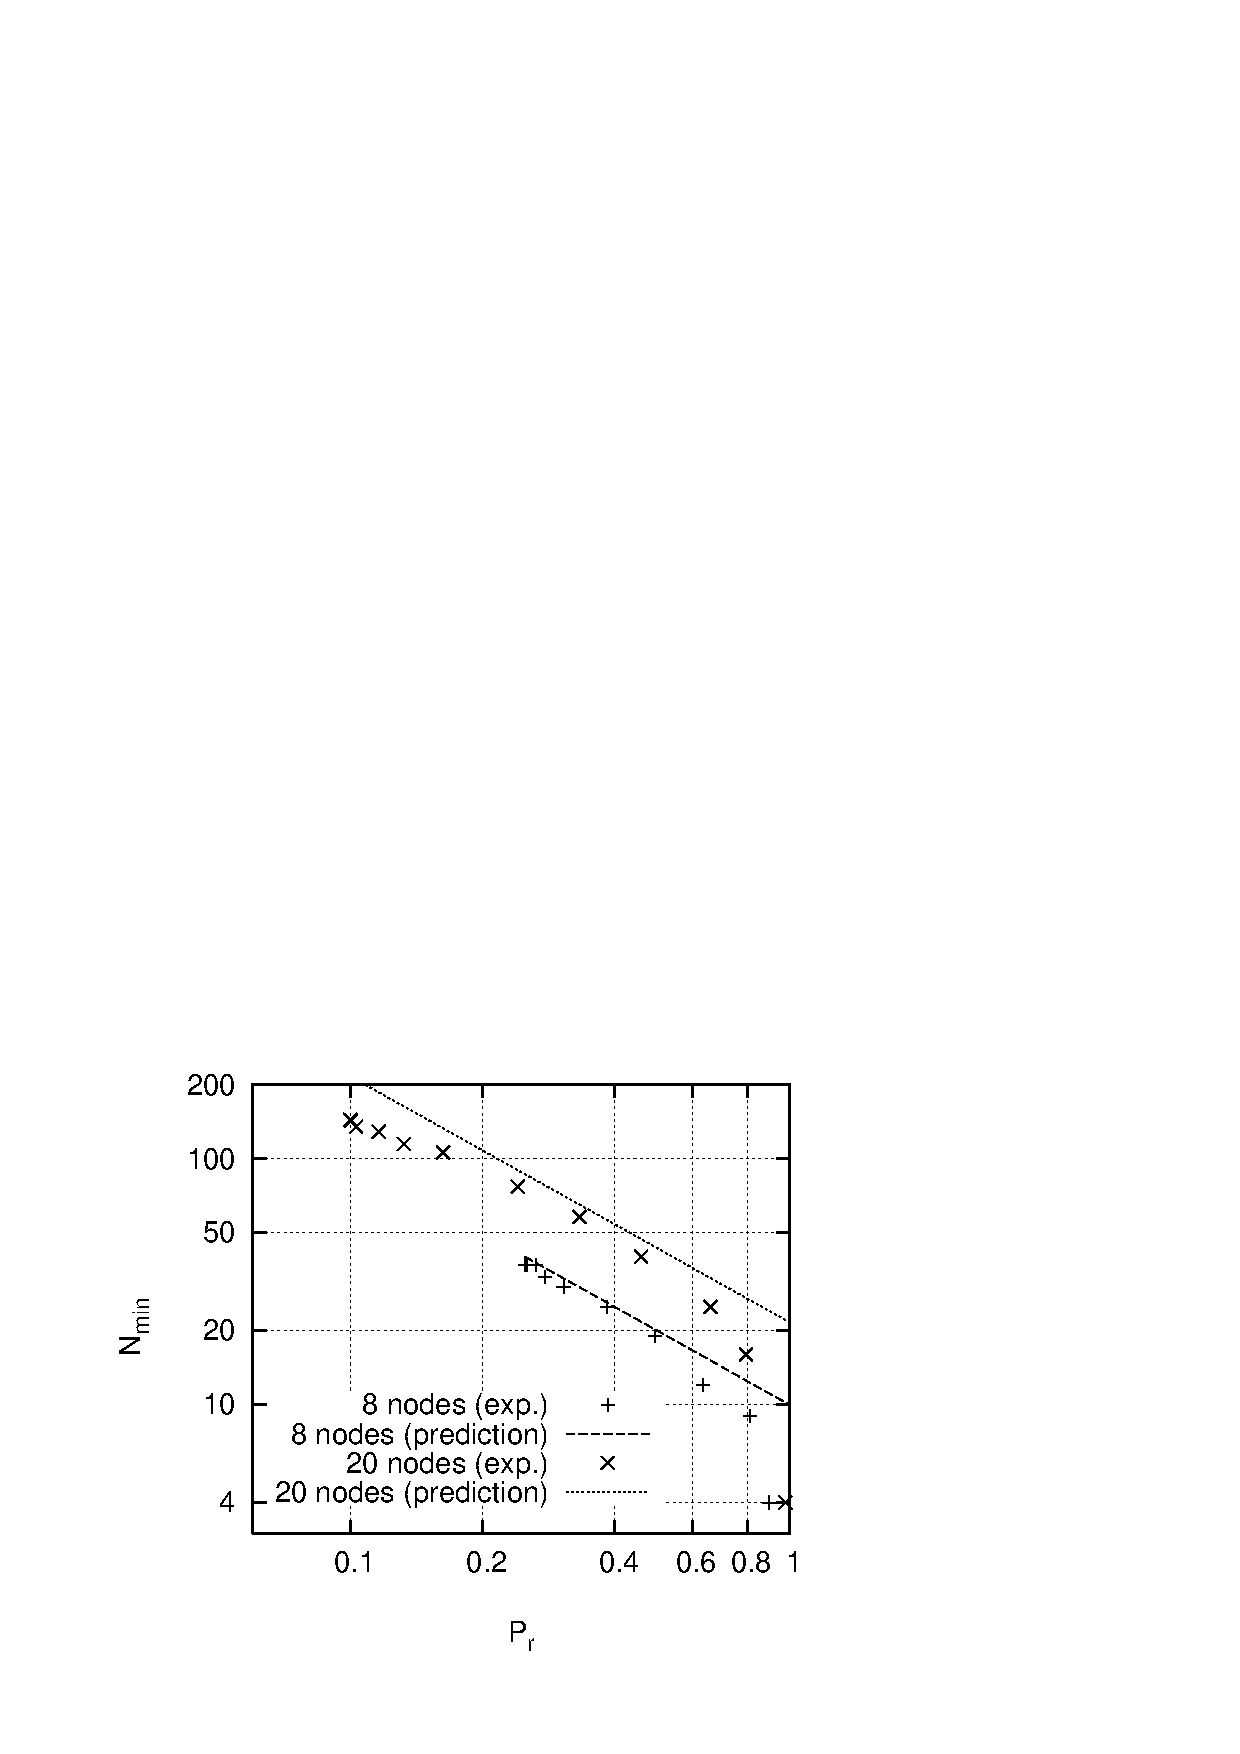
\includegraphics[width=\columnwidth]{grafiken/n-over-r8-20}
        }
\subfigure[Ein mit xfig erzeugtes Bild\label{fig:bild2}]
        {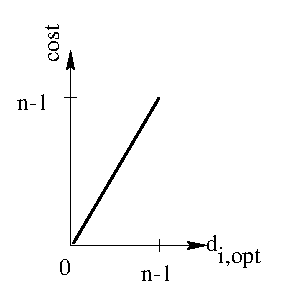
\includegraphics[width=3cm]{grafiken/cost}} 
\caption[Das hier steht im Abbildungsverzeichnis.]{Beispiele f{\"u}r sch{\"o}ne Bilder.\label{fig:bild1-und-bild2}}

\end{figure}


\section{Editor}

Als Editor f{\"u}r Fortgeschrittene ist xemacs gut geeignet.
Bei Verwendung von xemacs ist der Gebrauch der reftex und auctex-pakete zu empfehlen.
Als Rechtschreibprogramm sollte aspell verwendet werden und folgender Code in init.el eingef{\"u}gt werden.


 (require 'iso-cvt)\\
  (add-hook 'LaTeX-mode-hook\\
    (function (lambda ()\\
      ;; Setze Anfuehrungszeichen etc. fuer Style german\\
      (TeX-run-style-hooks "german")\\
      ;;\\
      ;; Lade Buffer und wandle nach ISO Latin-1:\\
      (format-encode-buffer 'plain)\\
      )))\\
\\
      (setq ispell-silently-savep t) ;save new words in pdict without questioning\\
(setq ispell-help-in-bufferp 'electric) ;get a better help buffer\\
(setq ispell-program-name "aspell")\\
(setq ispell-extra-args '("-W" "2"))\\
\\
(column-number-mode t)\\
\\
(custom-set-variables\\
 '(paren-mode 'sexp nil (paren)))\\
\\
 (setq reftex-plug-into-AUCTeX t)\\
(require 'reftex "reftex" t)\\
 (turn-on-reftex) ; use reftex\\
\\
 


Neulinge k{\"o}nnen auch einen sonstigen Editor oder Sachen wie Texnic Center, etc verwenden.

\section{Mathematik}

In latex kann man Formeln wundersch{\"o}n setzen.

\selectlanguage{english} % The following chapter is in english
As the following stuff is in English, we must change the hyphenation style.


The OCST problem is defined as follows. Let $G=(V,E)$ be a connected, undirected graph with $n=|V|$ nodes and $m=|E|$ edges. There are  communication, or transportation demands, between every pair of nodes.  An $n \times n$ {\em demand matrix} $R=(r_{ij})$ specifies the demands, where $r_{ij}$ is the amount of traffic required between location $v_i$ and $v_j$. Similarly, an $n\times n$ {\em distance matrix} $W=w_{ij}$ determines the distance weights between each pair of sites. 
A tree $T=(V,F)$ where $F \subseteq E$ and $|F|=|V|-1$ is called a {\em spanning tree} of $G$ if it connects all the nodes. The weight $w(T)$ of the spanning tree is the weighted sum over all pairs of vertices of the cost of the path between the pair in $T$. The communication cost over the tree $T$ is defined as 
\begin{equation}
  \label{equ:1}
w(T)=\sum_{i,j\in V}w_{ij}b_{ij},
\end{equation}
where $B=b_{ij}$ denotes the traffic flowing directly and indirectly across the edge connecting nodes $i$ and $j$. It is calculated according to the structure of $T$. 
$T$ is the optimal communication spanning tree if $w(T)\leq w(T')$ for all other spanning trees $T'$. %For the experiments we assume that there is an unique optimum tree ($w_{ij}\neq w_{kl}\forall (i\neq k, j\neq l)$).
The OCST problem becomes the minimum spanning tree (MST) problem if $w(T)=\sum_{i,j\in V}w_{ij}$. Then, $T$ is the simple minimum spanning tree if $w(T)\leq w(T')$  for all other spanning trees $T'$.%, where $w(T)=\sum_{i,j\in V}w_{ij}$. 
%In most instances of the OCST problem, the cost $f(w_{ij},b_{ij})$ of each link connecting the nodes $i$ and $j$ is calculated as the product of the distances $w_{ij}$ times the overall traffic $b_{ij}$ running over the link, so that $f=w_{ij}b_{ij}$. 

Cayley's formula identifies the number of spanning trees on $n$ nodes as $n^{n-2}$ . Furthermore, there are $n$ different stars on a graph of $n$ nodes. The similarity between two spanning trees $T_i$ and $T_j$ can be measured using the distance   $d_{ij}\in\{0,1,\ldots,n-1\}$ as 
$$
d_{ij}=\frac{1}{2}\sum_{u,v\in V,u<v}|l^{i}_{uv}-l^{j}_{uv}|,
$$
where $l^{i}_{uv}$ is 1 if an edge from $u$ to $v$ exists in $T_i$ and 0 if it does not exist in $T_i$. The number of edges that two trees $T_i$ and $T_j$ have in common is $n-1-d_{ij}$.




\selectlanguage{ngerman} % deutsch

Ab jetzt wieder deutsche Trennung.

In Abbildung \ref{fig:2dnorm} gibt es noch ein Beispiel f{\"u}r ein Bild und in Tabelle \ref{tab:einfache-tabelle} gibt es ein einfaches Bild. Tabelle~\ref{tab8:results-testproblem-deceptive} stellt eine etwas kompliziertere Tabelle dar. 
\begin{figure}[htb]
        \begin{center}
        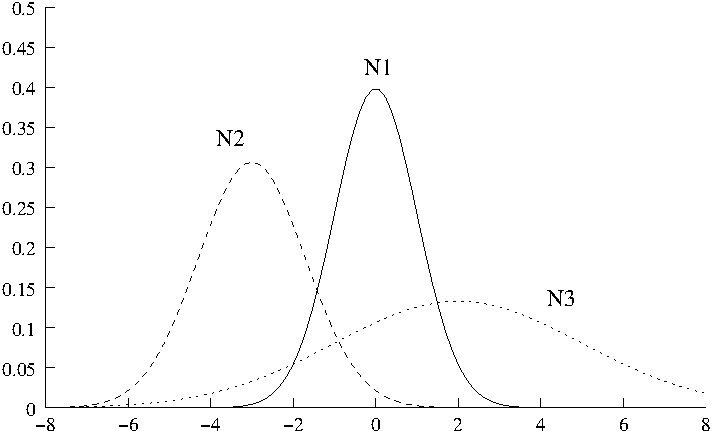
\includegraphics[width=8cm]{grafiken/norm_uni}
        \caption{Dichten univariater Normalverteilungen}
        \label{fig:2dnorm}
        \end{center}
\end{figure}


Beim Aufbau von Kommunikationsnetzen stehen Unternehmen vor dem Problem, eine Menge von unterschiedlichen Standorten so durch Leitungen zu verbinden, dass bestimmte Qualit{\"a}tsanforderungen (z.B. Sicherheit, Bandbreite, Zu\-ver\-l{\"a}ssig\-keit, Skalierbarkeit, etc.) eingehalten werden und gleichzeitig die Netzstruktur so gew{\"a}hlt wird, dass die Kosten des Netzaufbaus minimiert werden. Unternehmen, f{\"u}r welche der Aufbau von Kommunikationsnetzwerken relevant ist, lassen sich in zwei Gruppen unterteilen:

Auf der einen Seite sind Unternehmen zu finden, f{\"u}r die Kommunikationsnetzwerke ein wichtiger Teil ihrer Unternehmensinfrastruktur sind (z.B. Banken, Verlagsh{\"a}user, Bahn, Bundeswehr, Unternehmen mit mehreren Niederlassungen, etc.) und welche daher die Kommunikationsnetzwerke oft selbst betreiben. Ein Beispiel hierf{\"u}r ist die DATEV eG, welche {\"u}ber ein eigenes \glqq Genossenschaftsnetz'' mehrere Dutzend Niederlassungen an die Zentrale in N{\"u}rnberg anbindet. {\"U}ber dieses Kommunikationsnetz wird sowohl der gesamte Daten- als auch Telefonverkehr innerhalb des Unternehmens abgewickelt.


Auf der anderen Seite stehen Unternehmen, f{\"u}r die der Aufbau und der Betrieb von Kommunikationsnetzwerken Kernaufgaben darstellen (z.B. Telekommunikationsunternehmen (Deutsche Telekom oder Deutsches Forschungsnetz (DFN)), Mobilfunkbetreiber (vodafon, T-mobil) oder lokale Provider (NetCologne, Stadtwerke). F{\"u}r derartige Unternehmen geh{\"o}rt der Aufbau und Betrieb von Kommunikationsnetzwerken zum Kerngesch{\"a}ft. Netzwerke sind so aufzubauen und weiterzuentwickeln, dass Qualit{\"a}tskriterien eingehalten werden und gleichzeitig die Betriebskosten minimiert werden. 





\begin{table}
\caption{Eine sehr einfache Tabelle\label{tab:einfache-tabelle}}
\begin{center}
\begin{tabular}{|l|c|r|}
\hline
linksb{\"u}ndig & zentriert & rechtsb{\"u}ndig \\
\hline
1 & 2 & 3,141\\
\hline
\end{tabular}
\end{center}
\end{table}

Beim Aufbau von Kommunikationsnetzwerken kann unterschieden werden zwischen vermaschten und baumf{\"o}rmigen Netzwerken (vergleiche Abbildung \ref{fig:2dnorm}). In  vermaschten Netzen existieren mehrere unterschiedliche Wege f{\"u}r den Transport von Daten zwischen zwei Standorten. Daher muss bei vermaschten Netzwerken das Routing der Daten durch das Netzwerk gesteuert werden (wie z.B. im Internet). In der Regel existieren mehrere Wege zwischen zwei Standorten und es muss mit Hilfe von Routingmechanismen festgelegt werden, welchen Weg die Daten durch das Netz nehmen sollen (wie z.B. durch Routingtabellen f{\"u}r den IP-Verkehr im Internet). Diese Entscheidung wird unter anderem durch die Entfernung von Standorten als auch durch die Auslastung der unterschiedlichen Leitungen beeinflusst. Die Ermittlung von Routingtabellen ist in der Praxis recht aufwendig und es besteht die Gefahr, dass Nachrichten Umwege durch das Netz nehmen oder sogar im Kreis laufen. Vermaschte Netzwerke bieten allerdings eine erh{\"o}hte Ausfallsicherheit, da beim Vorhandensein von mehreren Wegen zwischen zwei Knoten Daten auch dann noch ausgetauscht werden k{\"o}nnen, wenn ein Teil des Netzwerkes ausf{\"a}llt.



\begin{table}
\centering
\caption{Performance of GAs using different types of representations for deceptive tree problems of different sizes and with different $T_{opt}$ (arbitrary tree, MST, and star)\label{tab8:results-testproblem-deceptive}}

\begin{tabular}{c|l|c|cc|cc}

\multirow{3}{*}{\rotatebox{90}{$T_{opt}$}}  && \multicolumn{5}{c}{oder 3}\\ \cline{3-7}
 && \multirow{2}{*}{$P_{succ}$}& \multicolumn{2}{c|}{fitness}& \multicolumn{2}{c}{$t_{conv}$}\\
& & &$\mu$ & $\sigma$& $\mu$ & $\sigma$  \\ \noalign{\vskip\arrayrulewidth\hrule height 1pt}
%
\multirow{7}{*}{\rotatebox{90}{arbitrary tree}} & Pr{\"u}fer number & 0.54 & 0.49 & (0.6) & 26.0 & (8.6 \\ \cline{2-7}
 & NetKey & 0.78 & 0.23 & (0.4) & 23.0 & (6.0) \\ \cline{2-7}
 & LB ($P_1$=1)  & 0.09 & 1.69 & (0.8) & 19.5 & (7.6) \\
 & LB ($P_1$=20) & 0.82 & 0.18 & (0.4) & 23.3 & (6.1)  \\
 & $P_1$=$P_2$=1 & 0.12 & 1.24 & (0.6) & 27.4 & (8.0) \\ \cline{2-7}
 & heur. xover & 0 & 2.63 & (0.5) & 8.7 & (2.4)   \\
 & h. ini \& xover  & 0 & 3.88 & (0.1) & 0.4 & (0.4) \\
\end{tabular}
\end{table}


Baumf{\"o}rmige Netze stellen einen Sonderfall von vermaschten Kommunikationsnetzwerken dar. Hierbei existiert genau ein m{\"o}glicher Weg zwischen den Knoten im Netz. Daher muss keine Entscheidung {\"u}ber das Routing getroffen werden und Routingmechanismen zur Steuerung des Datenflusses entfallen. Allerdings haben baumf{\"o}rmige Netzwerke das Problem, dass durch den Ausfall einer Leitung ein Teil der Knoten nicht mehr erreichbar sind. Baumf{\"o}rmige Kommunikationsnetzwerke werden oft bei einer {\"u}berschaubaren Anzahl von Standorten wie z.B. in Local Area Networks (LAN) oder Unternehmensnetzwerken (\glqq Corporate Networks'') eingesetzt. Insbesondere Unternehmen, welche eigene Netzwerke betreiben (z.B. die DATEV eG), verwenden oft baum\-f{\"o}r\-mi\-ge Kommunikationsnetzwerkstrukturen wegen ihrer geringereren Komplexit{\"a}t. 

Das Problem des kostenminimalen Aufbaus von vermaschten bzw. baumf{\"o}rmigen Kommunikationsnetzen wurde schon sehr fr{\"u}hzeitig in der Literatur formalisiert und beschrieben. Beim \glqq network design problem'' soll diejenige Netzwerkstruktur bestimmt werden, welche alle Standorte miteinander verbindet, alle Kommunikationsanforderungen zwischen den einzelnen Standorten erf{\"u}llt und gleichzeitig minimale Kosten besitzt. Aus dem allgemeinen \glqq network design problem'' l{\"a}sst sich das \glqq optimal communication spanning tree'' (OCST)-Problem ableiten, bei welchem die Struktur des gew{\"u}nschten Netzwerkes baumf{\"o}rmig ist. Im folgenden Abschnitt soll n{\"a}her auf das OCST Problem eingegangen werden.



%%% Local Variables: 
%%% mode: latex
%%% TeX-master: "..\\da-beispiel"
%%% End: 

\chapter{Discussion, Conclusions, and Further Work}
\label{chap:conclusions}
The purpose of this book is to understand  the influence of representations on the performance of genetic and evolutionary algorithms. 
This chapter summarizes the work contained in this study and lists its major contributions.


\section{Discussion}
\label{sec:discussion}

This is the final section \ref{sec:summary}. We  started in Chap.~\ref{chap:howto} by providing the necessary background for examining representations for  GEAs. Researchers recognized early that representations have a large influence on the performance of GEAs. Consequently, after a brief introduction into representations and GEAs, we discussed how the influence of representations on problem difficulty  can be measured. The chapter ended with prior guidelines for choosing high-quality  representations. Most of them are  mainly based on empirical observations and intuition and not on theoretical analysis.

Therefore, we presented in Chap.~\ref{cha:grafiken} three aspects of a theory of representations for  GEAs. We investigated how the locality, scaling, and locality of an encoding  influences GEA performance. The performance of GEAs is determined by the solution quality at the end of a run and the number of generations until the population is converged. Consequently, for redundant and exponentially scaled encodings, we presented population sizing models and described how the time to convergence is changed.
Furthermore, we were able to demonstrate that high-locality encodings do not change the difficulty of a problem; in contrast, when using low-locality encodings, on average, the difficulty of problems changes. Therefore,  easy problems become more difficult and difficult problems become easier by the use of low-locality encodings.
For all three properties of encodings, the theoretical models were verified with empirical results.


\section{Conclusions}
We  summarize the most important contributions of this work.

{\bf Framework for design and analysis of representations (and operators) for GEAs.} The main purpose of this study was to present a  framework which describes how genetic representations influence the performance of GEAs. The performance of GEAs is measured by the solution quality at the end of the run and the number of generations until the population is converged. 
The proposed framework allows us to analyze the influence of existing representations on GEA performance and to develop efficient new representations in a theory-guided way.
Furthermore, we illustrated that the framework can also be used for the design and analysis of search operators, which are relevant for direct encodings.
Based on the framework, the development of high-quality representations remains not only a matter of intuition and random search but becomes an engineering design task.
Even though more work is needed, we believe that the results presented are sufficiently compelling to recommend increased use of the framework.



{\bf Redundancy, Scaling, and Locality}. These are the three elements of the proposed framework of representations.  We demonstrated that these three properties of representations influence GEA performance and presented theoretical models to predict how solution quality and time to convergence changes.
By examining the redundancy, scaling, and locality of an encoding, we are able to predict the influence of representations on GEA performance.

The theoretical analysis shows that the redundancy of an encoding influences the supply of building blocks (BB) in the initial population. $r$ denotes the number of genotypic BBs that represent the best phenotypic BB, and $k_r$ denotes the order of redundancy. For synonymously redundant encodings, where all genotypes that represent the same phenotype are similar to each other, the probability of GEA failure goes either with  $O(\exp(-r/2^{k_r}))$ (uniformly scaled representations) or  with $O(\exp(-\sqrt{r/2^{k_r}}))$ (exponentially scaled representations).
Therefore, GEA performance increases if the representation overrepresents high-quality BBs. If a representation is uniformly redundant, that means each phenotype is represented by the same number of genotypes, GEA performance remains unchanged in comparison to non-redundant encodings.

The analysis of the scaling of an encoding reveals that non-uniformly scaled representations modify the dynamics of genetic search. If exponentially scaled representations are used, the alleles are solved serially which increases the overall time until convergence and results in problems with genetic drift but allows rough approximations of the expected optimal solution after a few generations.

We know from previous work that the high locality of an encoding is a necessary condition for efficient mutation-based search.
An encoding has high locality if neighboring phenotypes correspond to neighboring genotypes.
Investigating the  influence of locality shows that  high-locality encodings do not change the difficulty of a problem. In contrast, low-locality encodings, where phenotypic neighbors do not correspond to genotypic neighbors, change problem difficulty and make, on average, easy problems more difficult and deceptive problems easier.
Therefore, to assure that  an easy problem remains easy, high-locality representations  are necessary.

\section{Further Work}

What are the open questions? What should be done next?




%%% Local Variables: 
%%% mode: latex
%%% TeX-master: "..\\da-beispiel"
%%% End: 

%\selectlanguage{ngerman} % wenn im Inhaltsverzeichnis Appendix stehen soll, muss Engl gewaehlt sein, fuer Anhang Deutsch
\appendix

%Bibliographie
%waehle einen der folgenden 4 Eintraege
%\bibliographystyle{literatur/natdin} %DIN Style Literaturverzeichnis, comment out pagebackref
%\bibliographystyle{literatur/IEEEtran} % IEEE Style Literaturverzeichnis
%\bibliographystyle{literatur/natdinCustomized} %DIN Style Literaturverzeichnis + Punkt hinter jeder Literaturangabe -> low level config fuer Zitate: natdin.cfg im Projektordner, comment out pagebackref
%\bibliographystyle{literatur/natdinCustomizedEnglish} %DIN Style auf Englisch getrimmt mit Punkt hinter Literaturangabe -> low lovel config fuer Zitate: natdin.cfg im Projektordner, pagebackref kann damit nicht genutzt werden
%\bibliographystyle{aer} % alternativ auch apalike, aer, apalike2... s.a. http://web.reed.edu/cis/Help/LaTeX/bibtexstyles.html
\bibliographystyle{apalike2} % very nice bib style
%note on aer: does not like inbook entries
%\bibliographystyle{natdin}

\bibliography{literatur/lit} %Pfad zur bib-Datei

%appendices can be defined here, the appendix structure has to be added manually to the toc (table of contents)
%\clearpage  %toc new page
%\addcontentsline{toc}{chapter}{Appendix} %add chapter to toc
\addpart{\appendixname}
\chapter{Simile - Code}
\label{append:simile-code}
In this section we will expose the different Java classes of our prototype.

\section{de.unimannheim.informatik.swt.simile}
\lstinputlisting[
  language=Java, numbers=left, stepnumber=5, firstnumber=1, breaklines=true, 
  basicstyle=\footnotesize,
  numberstyle=\tiny,
  caption={Simile.java},
  captionpos=b,
  label=Simile.java
]
{code/main/Simile.java.txt}

\lstinputlisting[
  language=Java, numbers=left, stepnumber=5, firstnumber=1, breaklines=true, 
  basicstyle=\footnotesize,
  numberstyle=\tiny,
  caption={ServletInitializer.java},
  captionpos=b,
  label=ServletInitializer.java
]
{code/main/ServletInitializer.java.txt}

\lstinputlisting[
  language=Java, numbers=left, stepnumber=5, firstnumber=1, breaklines=true, 
  basicstyle=\footnotesize,
  numberstyle=\tiny,
  caption={SimileApplication.java},
  captionpos=b,
  label=SimileApplication.java
]
{code/main/SimileApplication.java.txt}
\subsection{de.unimannheim.informatik.swt.simile.controllers}
\lstinputlisting[
  language=Java, numbers=left, stepnumber=5, firstnumber=1, breaklines=true, 
  basicstyle=\footnotesize,
  numberstyle=\tiny,
  caption={EntryController.java},
  captionpos=b,
  label=EntryController.java
]
{code/controller/EntryController.java.txt}
\subsection{de.unimannheim.informatik.swt.simile.model}
\lstinputlisting[
  language=Java, numbers=left, stepnumber=5, firstnumber=1, breaklines=true, 
  basicstyle=\footnotesize,
  numberstyle=\tiny,
  caption={Candidate.java},
  captionpos=b,
  label=Candidate.java
]
{code/model/Candidate.java.txt}

\lstinputlisting[
  language=Java, numbers=left, stepnumber=5, firstnumber=1, breaklines=true, 
  basicstyle=\footnotesize,
  numberstyle=\tiny,
  caption={Message.java},
  captionpos=b,
  label=Message.java
]
{code/model/Message.java.txt}

\lstinputlisting[
  language=Java, numbers=left, stepnumber=5, firstnumber=1, breaklines=true, 
  basicstyle=\footnotesize,
  numberstyle=\tiny,
  caption={Metric.java},
  captionpos=b,
  label=Metric.java
]
{code/model/Metric.java.txt}
\subsection{de.unimannheim.informatik.swt.simile.services}
\lstinputlisting[
  language=Java, numbers=left, stepnumber=5, firstnumber=1, breaklines=true, 
  basicstyle=\footnotesize,
  numberstyle=\tiny,
  caption={Cloner.java},
  captionpos=b,
  label=Cloner.java
]
{code/services/Cloner.java.txt}

\lstinputlisting[
  language=Java, numbers=left, stepnumber=5, firstnumber=1, breaklines=true, 
  basicstyle=\footnotesize,
  numberstyle=\tiny,
  caption={DirectoryExplorer.java},
  captionpos=b,
  label=DirectoryExplorer.java
]
{code/services/DirectoryExplorer.java.txt}

\lstinputlisting[
  language=Java, numbers=left, stepnumber=5, firstnumber=1, breaklines=true, 
  basicstyle=\footnotesize,
  numberstyle=\tiny,
  caption={EmailSender.java},
  captionpos=b,
  label=EmailSender.java
]
{code/services/EmailSender.java.txt}

\lstinputlisting[
  language=Java, numbers=left, stepnumber=5, firstnumber=1, breaklines=true, 
  basicstyle=\footnotesize,
  numberstyle=\tiny,
  caption={FileHandler.java},
  captionpos=b,
  label=FileHandler.java
]
{code/services/FileHandler.java.txt}

\lstinputlisting[
  language=Java, numbers=left, stepnumber=5, firstnumber=1, breaklines=true, 
  basicstyle=\footnotesize,
  numberstyle=\tiny,
  caption={Filter.java},
  captionpos=b,
  label=Filter.java
]
{code/services/Filter.java.txt}

\lstinputlisting[
  language=Java, numbers=left, stepnumber=5, firstnumber=1, breaklines=true, 
  basicstyle=\footnotesize,
  numberstyle=\tiny,
  caption={JavaClassFilter.java},
  captionpos=b,
  label=JavaClassFilter.java
]
{code/services/JavaClassFilter.java.txt}

\lstinputlisting[
  language=Java, numbers=left, stepnumber=5, firstnumber=1, breaklines=true, 
  basicstyle=\footnotesize,
  numberstyle=\tiny,
  caption={JavaClassHandler.java},
  captionpos=b,
  label=JavaClassHandler.java
]
{code/services/JavaClassHandler.java.txt}

\lstinputlisting[
  language=Java, numbers=left, stepnumber=5, firstnumber=1, breaklines=true, 
  basicstyle=\footnotesize,
  numberstyle=\tiny,
  caption={JavaClassVisitor.java},
  captionpos=b,
  label=JavaClassVisitor.java
]
{code/services/JavaClassVisitor.java.txt}

\lstinputlisting[
  language=Java, numbers=left, stepnumber=5, firstnumber=1, breaklines=true, 
  basicstyle=\footnotesize,
  numberstyle=\tiny,
  caption={JavaMethodVisitor.java},
  captionpos=b,
  label=JavaMethodVisitor.java
]
{code/services/JavaMethodVisitor.java.txt}

\lstinputlisting[
  language=Java, numbers=left, stepnumber=5, firstnumber=1, breaklines=true, 
  basicstyle=\footnotesize,
  numberstyle=\tiny,
  caption={NodeIterator.java},
  captionpos=b,
  label=NodeIterator.java
]
{code/services/NodeIterator.java.txt}

\lstinputlisting[
  language=Java, numbers=left, stepnumber=5, firstnumber=1, breaklines=true, 
  basicstyle=\footnotesize,
  numberstyle=\tiny,
  caption={SocoraRequester.java},
  captionpos=b,
  label=SocoraRequester.java
]
{code/services/SocoraRequester.java.txt}
\subsection{de.unimannheim.informatik.swt.simile.util}
\lstinputlisting[
  language=Java, numbers=left, stepnumber=5, firstnumber=1, breaklines=true, 
  basicstyle=\footnotesize,
  numberstyle=\tiny,
  caption={StreamGobbler.java},
  captionpos=b,
  label=StreamGobbler.java
]
{code/util/StreamGobbler.java.txt}

\chapter{Installation of Simile}
In this chapter we will show how to install the tools we used for implementing Simile. First we will start installing the CI Server Jenkins and explain how to configure it. Then, we will continue with installing Simile Jenkins plugin. After that we will explain how to configure Simile Jenkins plugin using the test project.

\section{Installation of Jenkins}
In this section we will explain how to install Jenkins CI server using Docker.

\subsection{Docker}
For installing Jenkins, we will use Docker containers and in this subsection we will explain how to install it in different platform such as macOS and Linux.

\subsubsection{Docker on macOS}
For macOS we will use Docker for Mac tool. This is an integrated, easy-to-deploy environment for building, assembling, and shipping applications from a Mac. Moreover, it is a native Mac application architected from scratch, with a native user interface and auto-update capability, deeply integrated with OS X native virtualization, Hypervisor Framework, networking and file system, making it faster and more reliable than previous ways of getting Docker on a Mac \cite{Docker}.

First we will download the tool from the following link: \url{https://download.docker.com/mac/stable/Docker.dmg}.\\

After downloading the \textit{dmg} image, double-click on it and you will see something like figure \ref{fig:docker-mac-01}. When you get that image, drag and drop the Docker icon to the Applications folder. After that, go to Applications folder and double click on Docker application.

\begin{figure}[ht]
	\centering
    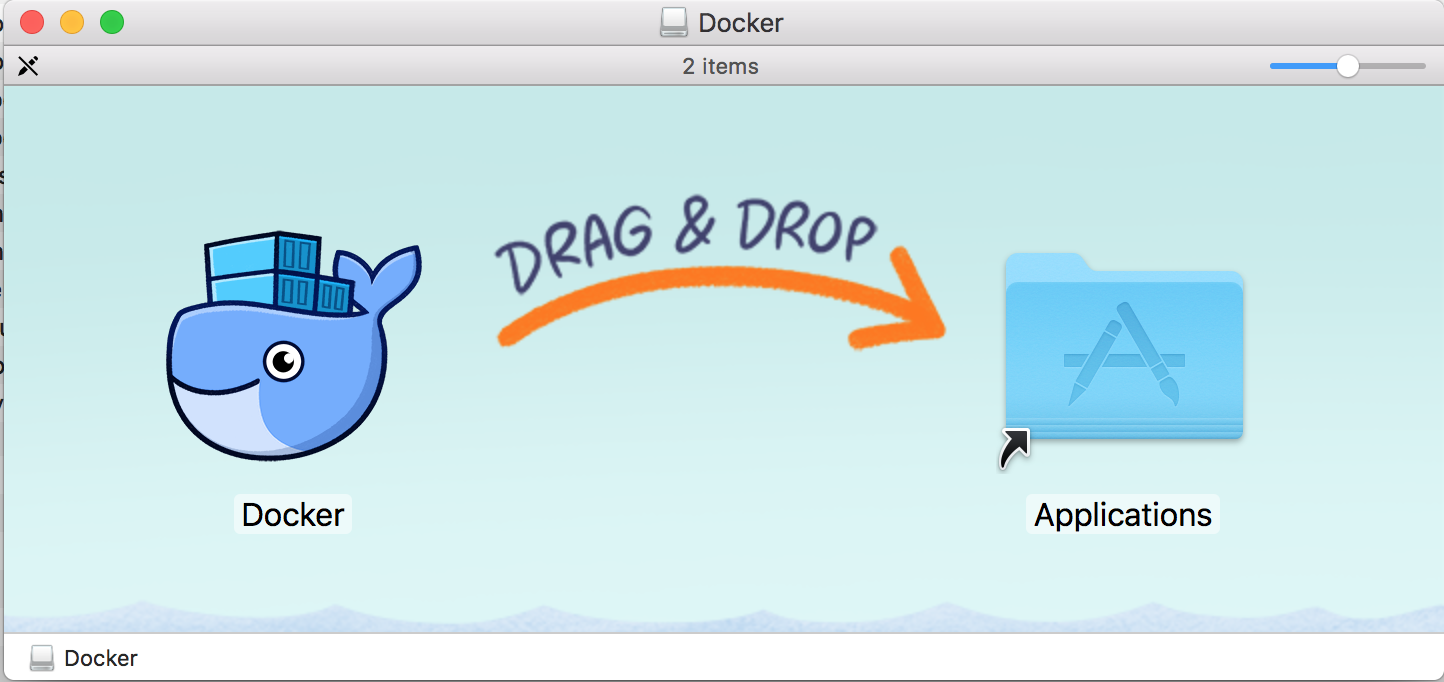
\includegraphics[width=\textwidth]{grafiken/docker-01}
    \caption{Docker for Mac installation}
    \label{fig:docker-mac-01}
\end{figure}

\subsubsection{Docker on Linux}
In this section we will explain how to install Docker in Linux, specifically in Debian (Jessie). For other distros please refer to Docker documentation\footnote{https://docs.docker.com/engine/installation/linux/ (accessed: 21.01.2017)}.

First of all we need to update the repositories.

\begin{minted}[linenos,
               numbersep=5pt,
               frame=lines,
               framesep=2mm]{bash}
$ sudo apt-get udpate
\end{minted}

Then we need to install the packages to allow \textit{apt} to use repositories iver HTTPS.

\begin{minted}[linenos,
               numbersep=5pt,
               frame=lines,
               framesep=2mm]{bash}
$ sudo apt-get install apt-transport-https \
                       ca-certificates \
                       software-properties-common
\end{minted}

Then we add the official Docker's GPG key.

\begin{minted}[linenos,
               numbersep=5pt,
               frame=lines,
               framesep=2mm]{bash}
$ curl -fsSL https://yum.dockerproject.org/gpg | sudo apt-key add -
\end{minted}

Finally we add the stable repository of Docker and update repositories.

\begin{minted}[linenos,
               numbersep=5pt,
               frame=lines,
               framesep=2mm]{bash}
$ sudo add-apt-repository \
       "deb https://apt.dockerproject.org/repo/ \
       debian-$(lsb_release -cs) \
       main"
$ sudo apt-get update
\end{minted}

Once we added the new repositories, we update the repository list.

\begin{minted}[linenos,
               numbersep=5pt,
               frame=lines,
               framesep=2mm]{bash}
$ sudo apt-get update
\end{minted}

Then we install docker.

\begin{minted}[linenos,
               numbersep=5pt,
               frame=lines,
               framesep=2mm]{bash}
$ sudo apt-get -y install docker-engine
\end{minted}

After the installation is done we can make a little test to be sure that everything was installed correctly. The following command will download a test image and runs it in a container. Once it is running will print an informational message and exits.

\begin{minted}[linenos,
               numbersep=5pt,
               frame=lines,
               framesep=2mm]{bash}
$ sudo docker run hello-world
\end{minted}

\subsection{Jenkins in Docker}
Open a terminal on your mac and enter the following command to download the Jenkins image for Docker.

\begin{minted}[linenos,
               numbersep=5pt,
               frame=lines,
               framesep=2mm]{bash}
$ docker pull jenkins
  Using default tag: latest
  latest: Pulling from library/jenkins

  # some irrelevant output was remove
  Digest: sha256:5046434030be395ec977c98e11...
  Status: Downloaded newer image for jenkins:latest
\end{minted}

Then, we just need to run the Jenkins image with the following command.

\begin{minted}[linenos,
               numbersep=5pt,
               frame=lines,
               framesep=2mm,
               breakanywhere]{bash}
$ docker run -p 8080:8080 -p 50000:50000 jenkins
  # some irrelevant output was remove
  *************************************************************

  Jenkins initial setup is required. An admin user has been 
  created and a password generated.
  Please use the following password to proceed to installation:

  95199411f1894bfa97e937147c41aa62 # IMPORTANT, default admin pass

  This may also be found at: /var/jenkins_home/secrets/initial.
 
  *************************************************************
  # some irrelevant output was removed
  Jan 19, 2017 8:28:05 AM hudson.model.AsyncPeriodicWork$1 run
  INFO: Finished Download metadata. 25,312 ms
\end{minted}

After that, open the following URL \url{http://localhost:8080} and you should see some like figure \ref{fig:jenkins-01}.

\begin{figure}[H]
	\centering
    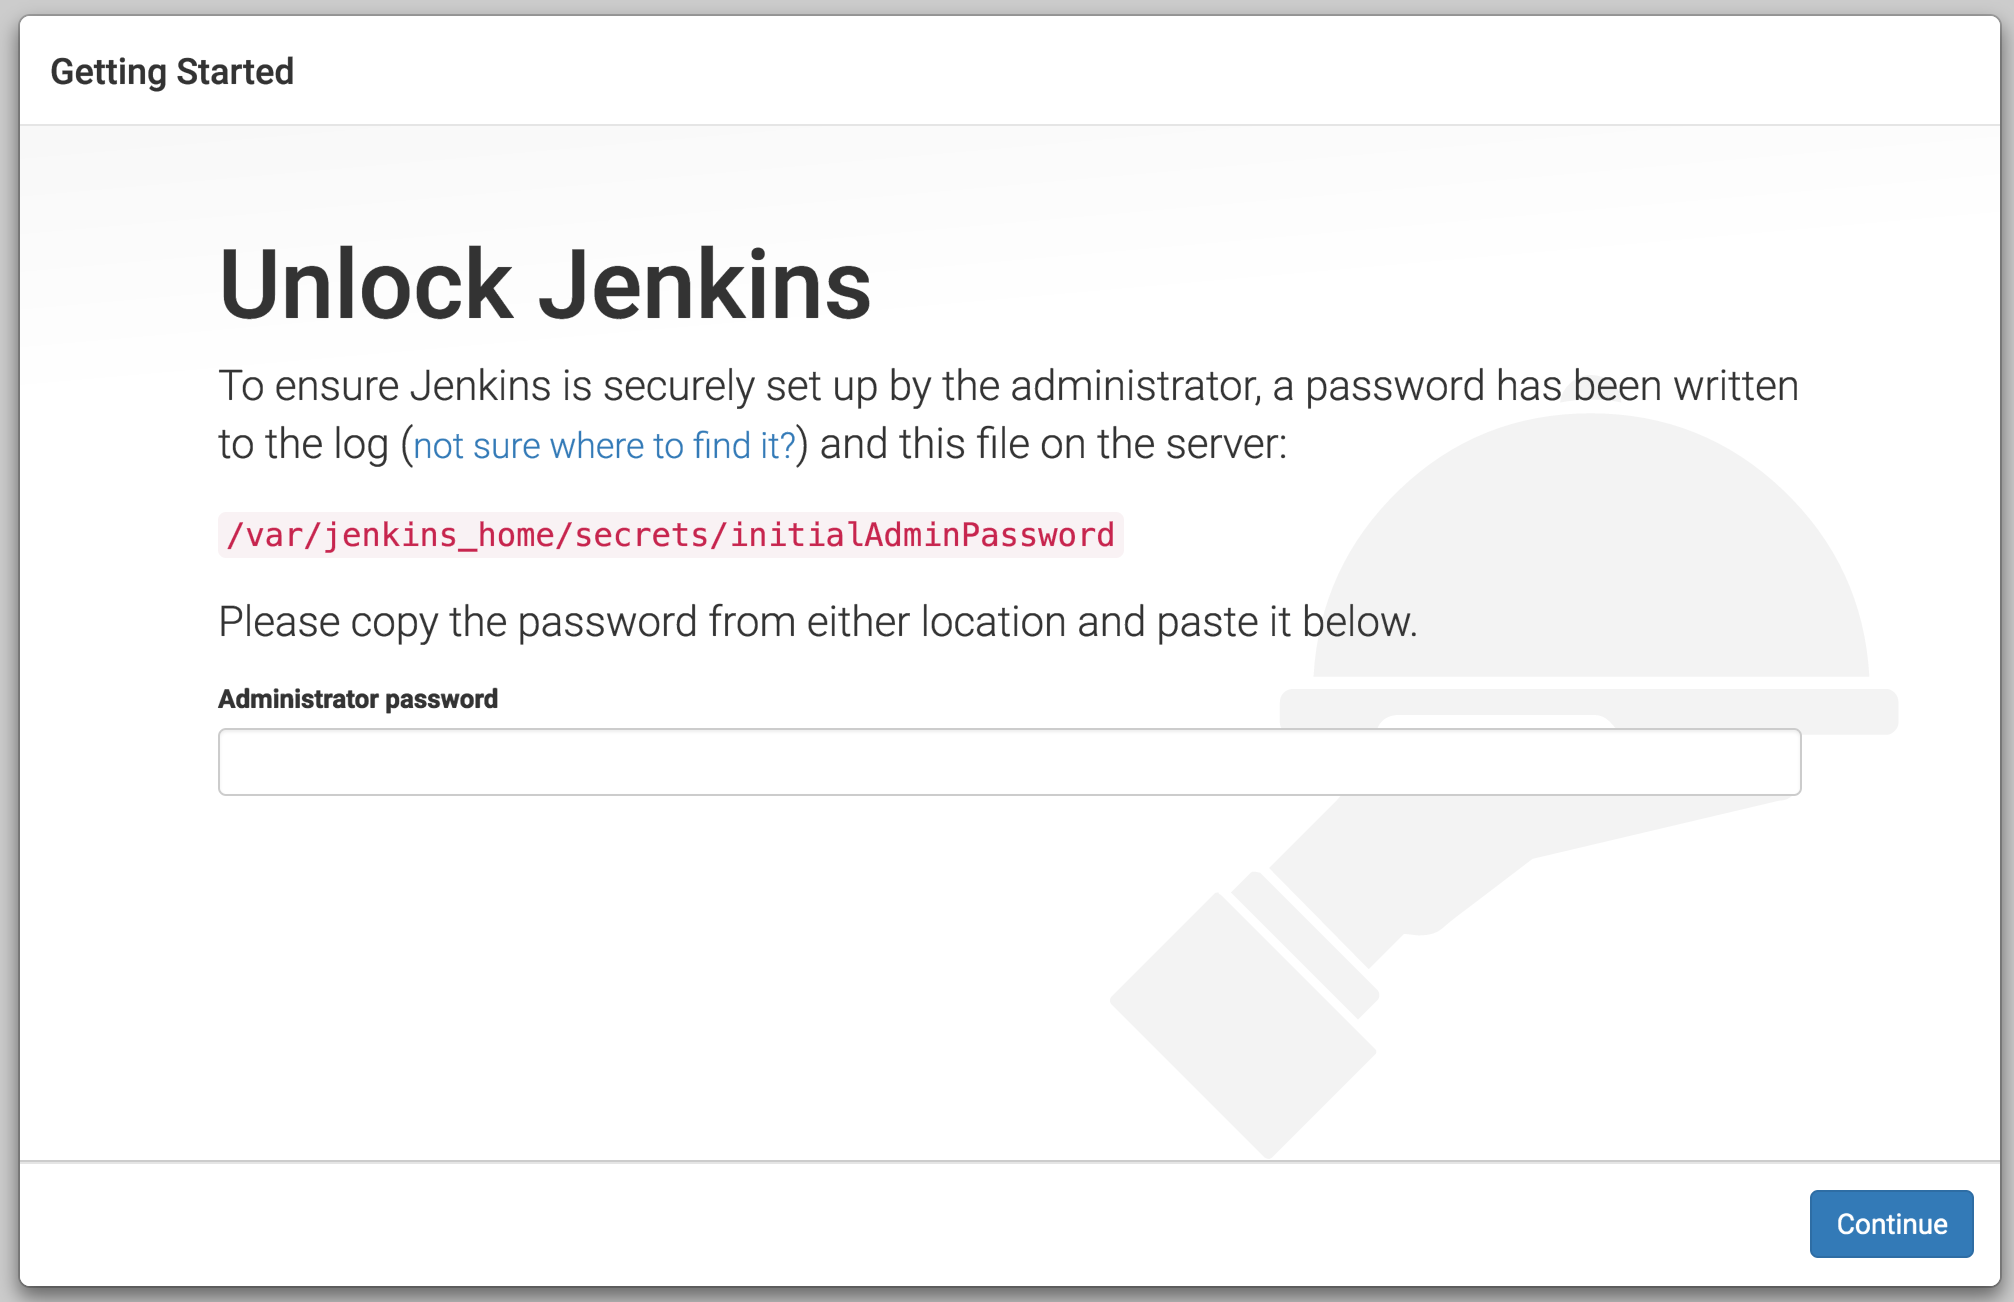
\includegraphics[width=0.7\textwidth]{grafiken/jenkins-01}
    \caption{First page of Jenkins setup}
    \label{fig:jenkins-01}
\end{figure}

There enter the password generated by Jenkins and that appeared in the logs, and then click on continue.

In the folowing page click on \textit{Install suggested plugins} like the figure \ref{fig:jenkins-02}.

\begin{figure}[H]
	\centering
    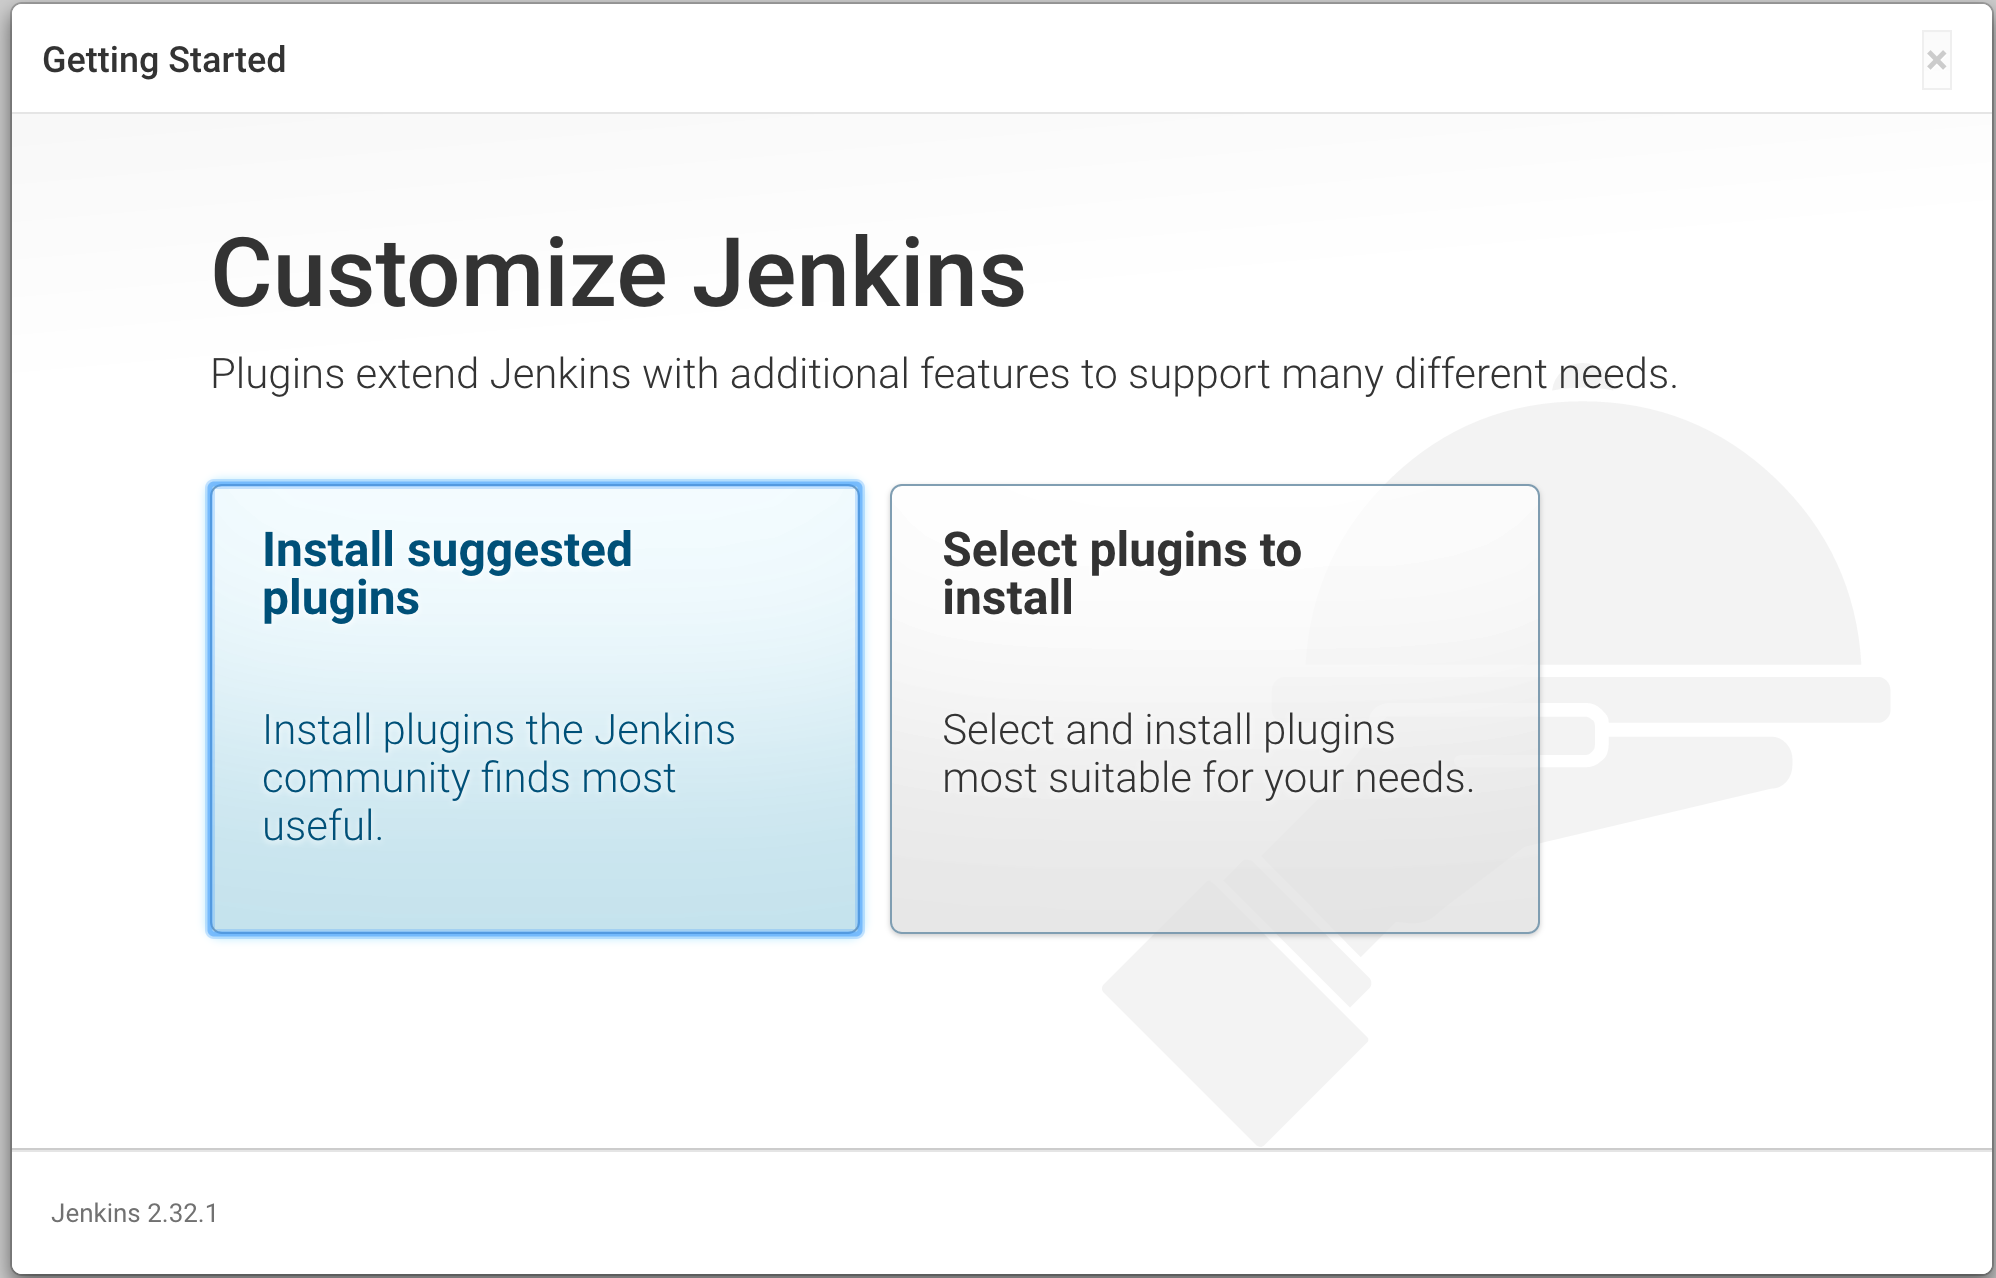
\includegraphics[width=0.8\textwidth]{grafiken/jenkins-02}
    \caption{Second page of Jenkins setup}
    \label{fig:jenkins-02}
\end{figure}

Then you should see something like the figure \ref{fig:jenkins-03}. Here we just need to wait untill the plugins installation finish.

\begin{figure}[H]
	\centering
    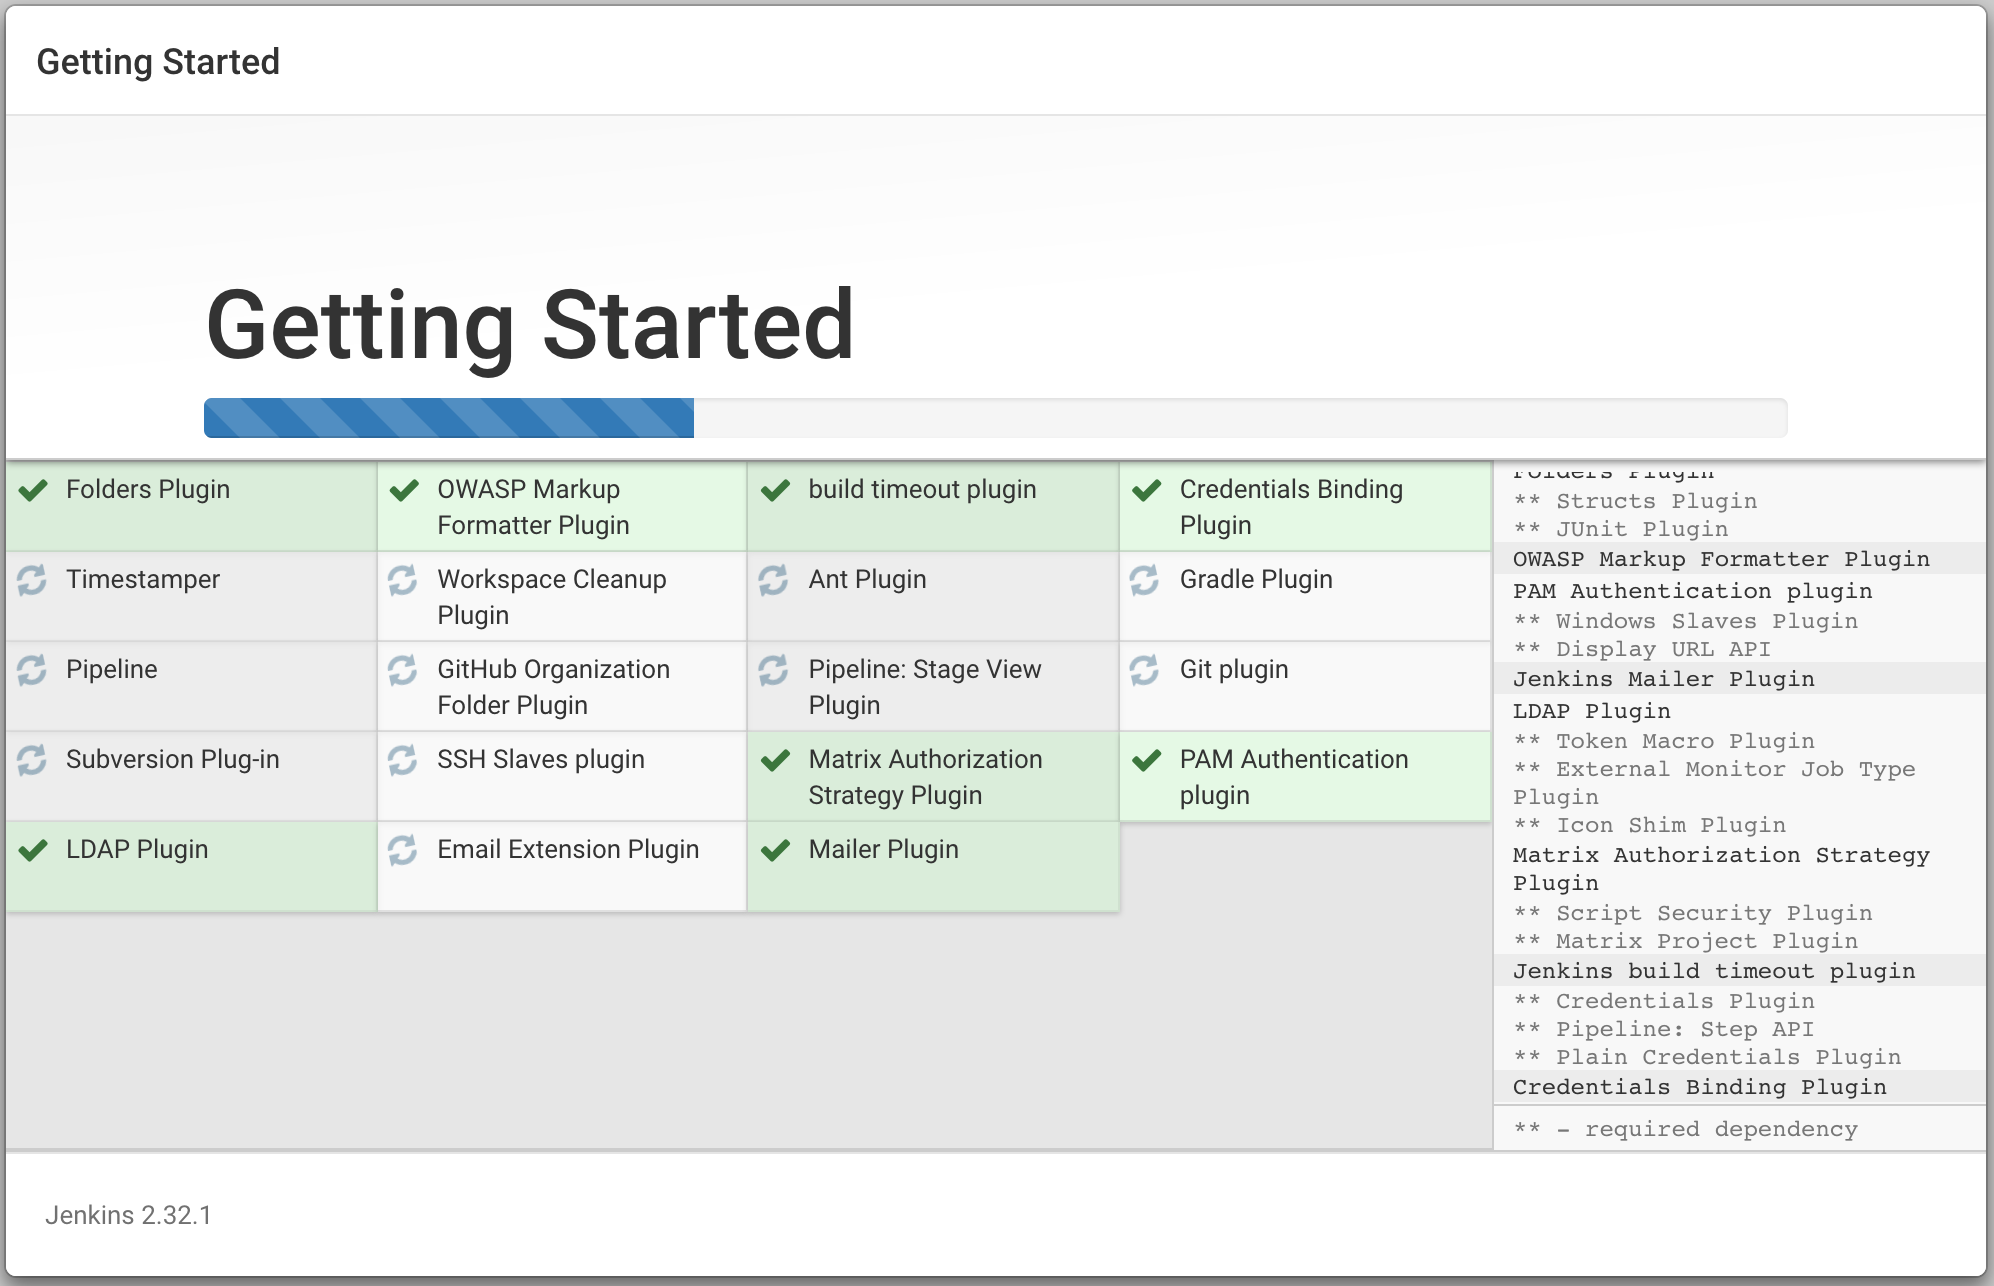
\includegraphics[width=0.8\textwidth]{grafiken/jenkins-03}
    \caption{Third page of Jenkins setup}
    \label{fig:jenkins-03}
\end{figure}

After the installation of plugins is done, click on \textit{Continue as admin} or create custom admin user. Then you should see the home page of Jenkins (figure )

\begin{figure}[H]
	\centering
    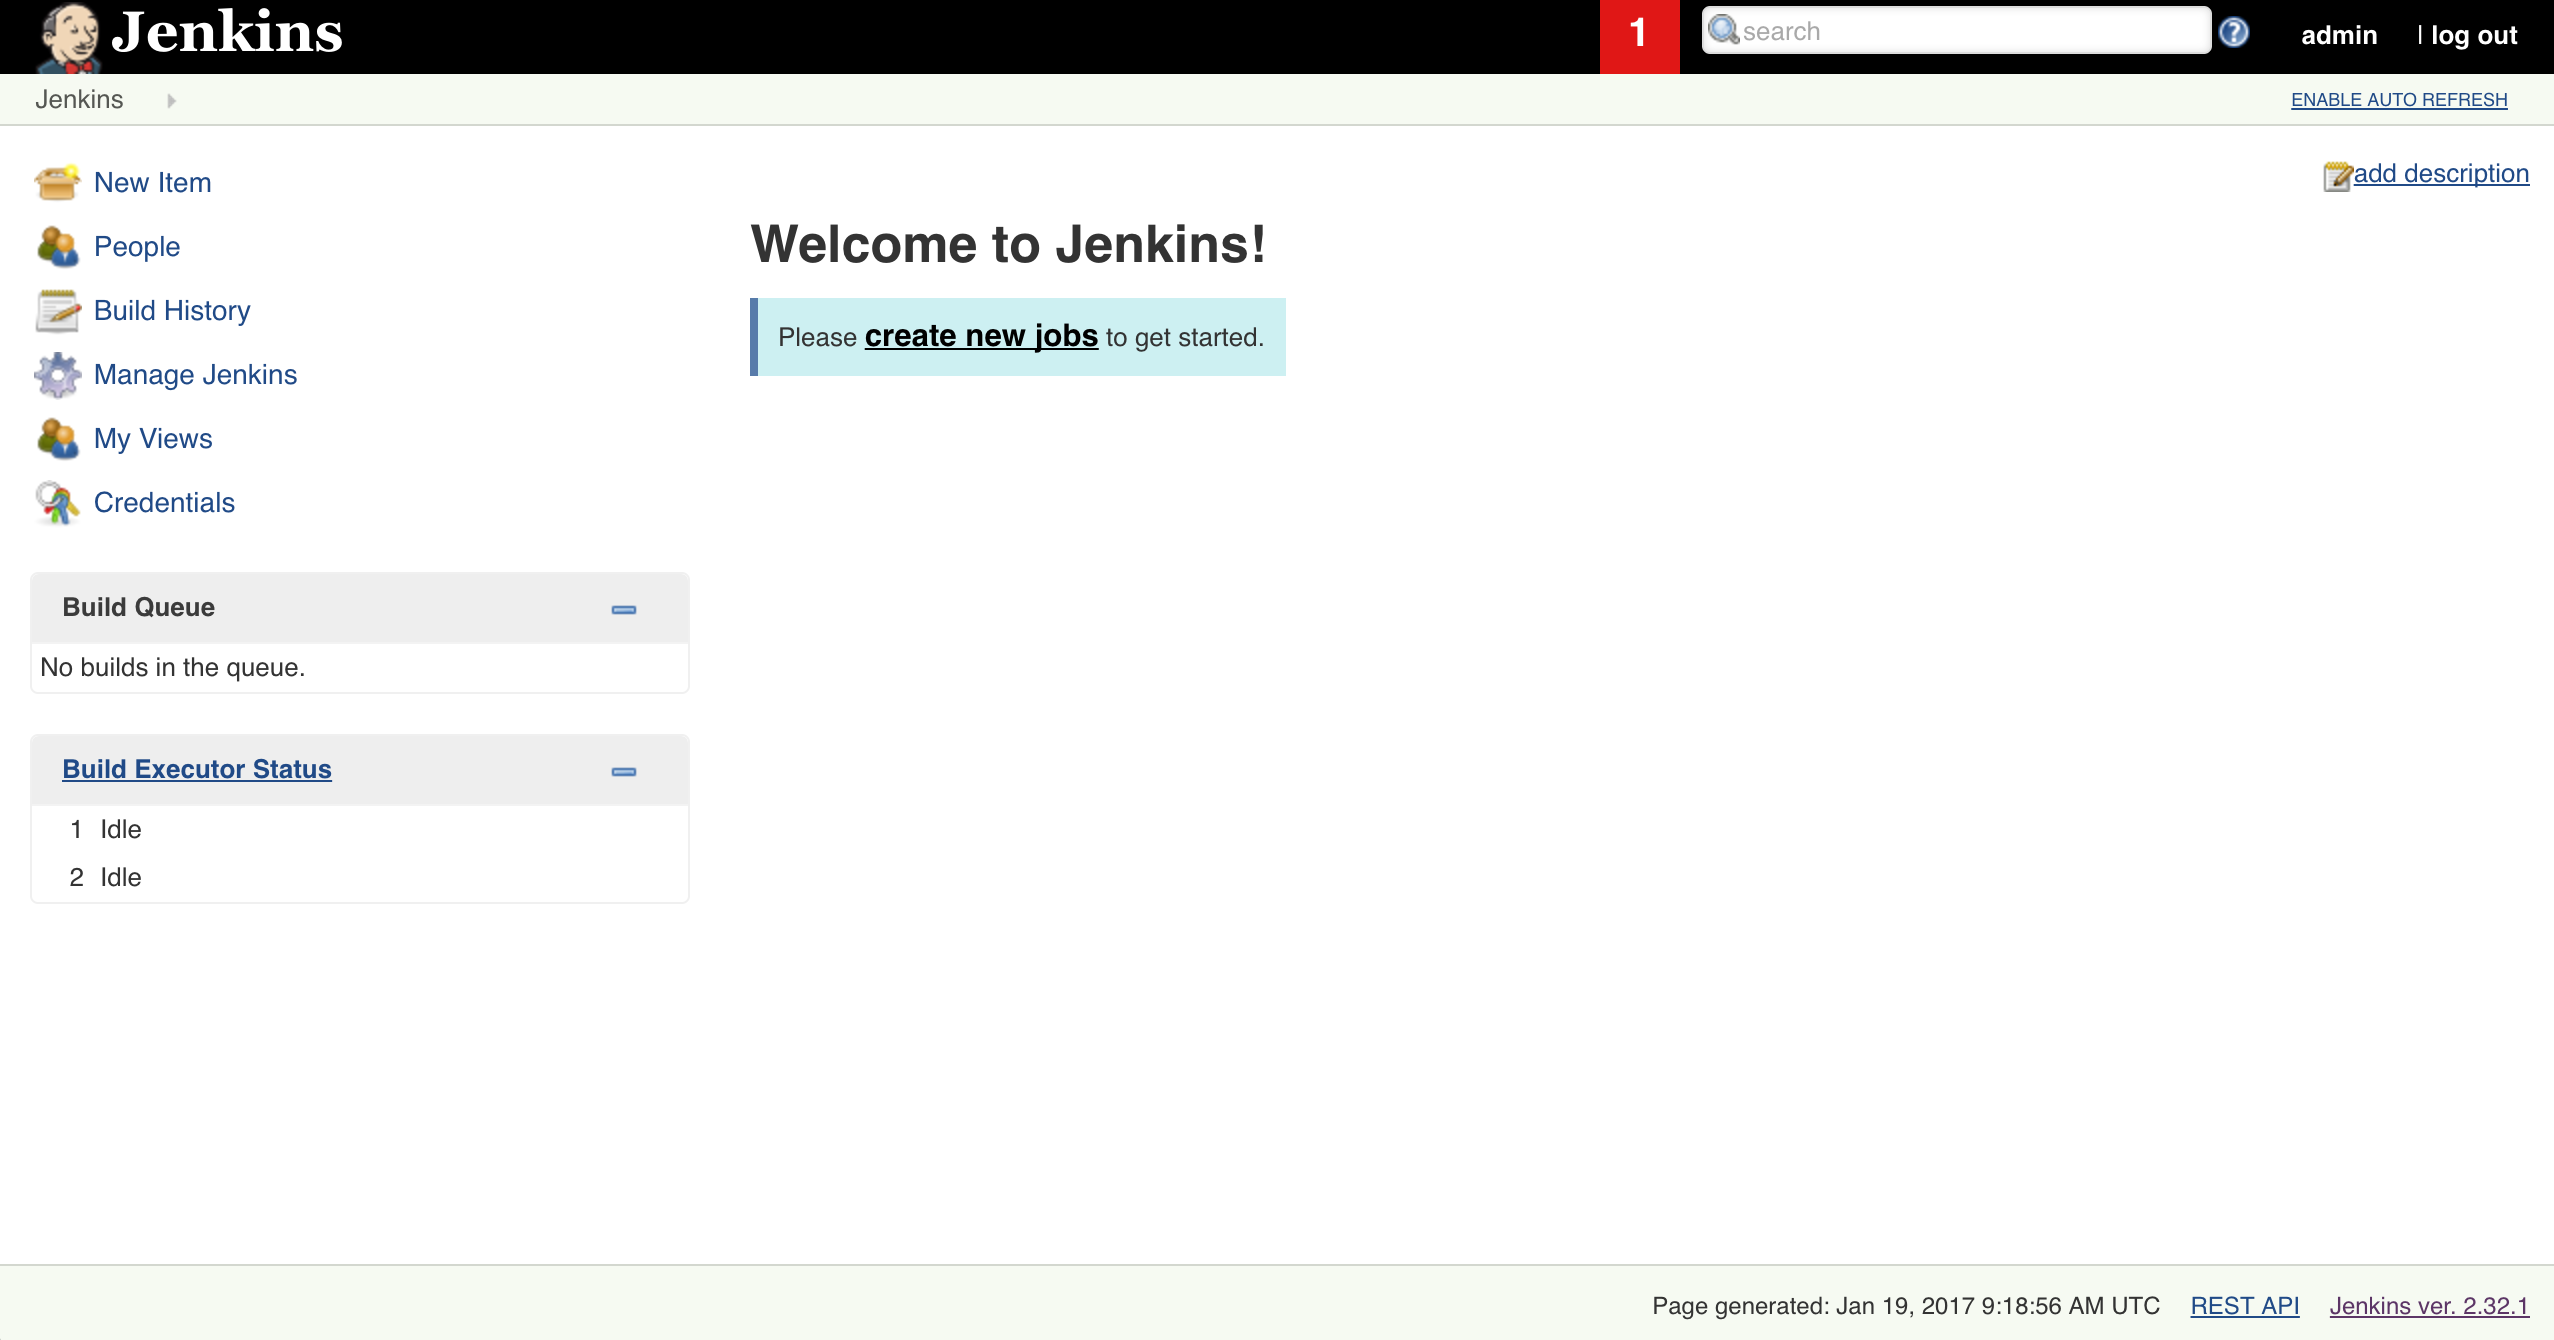
\includegraphics[width=0.8\textwidth]{grafiken/jenkins-04}
    \caption{Jenkins home page}
    \label{fig:jenkins-04}
\end{figure}

\section{Simile Jenkins Plugin installation}
To install Simile Jenkins plugin, we need to follow the following steps.

First, open Jenkins URL. Then click on \textit{Manage Jenkins} (figure \ref{fig:jenkins-plugin-01}).

\begin{figure}[H]
	\centering
    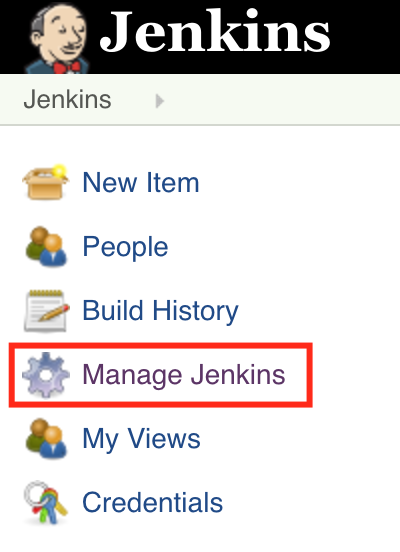
\includegraphics[width=0.25\textwidth]{grafiken/jenkins-plugin-01}
    \caption{Manage Jenkins option}
    \label{fig:jenkins-plugin-01}
\end{figure}

Then click on \textit{Manage Plugins} (figure \ref{fig:jenkins-plugin-02}).

\begin{figure}[H]
	\centering
    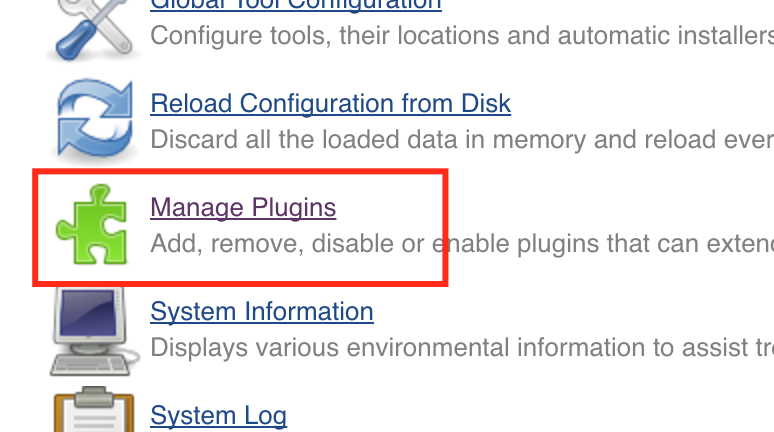
\includegraphics[width=0.5\textwidth]{grafiken/jenkins-plugin-02}
    \caption{Manage Plugins option}
    \label{fig:jenkins-plugin-02}
\end{figure}

Then go to \textit{Advanced}, scroll down until \textit{Upload Plugin} section (figure \ref{fig:jenkins-plugin-03}).

\begin{figure}[H]
	\centering
    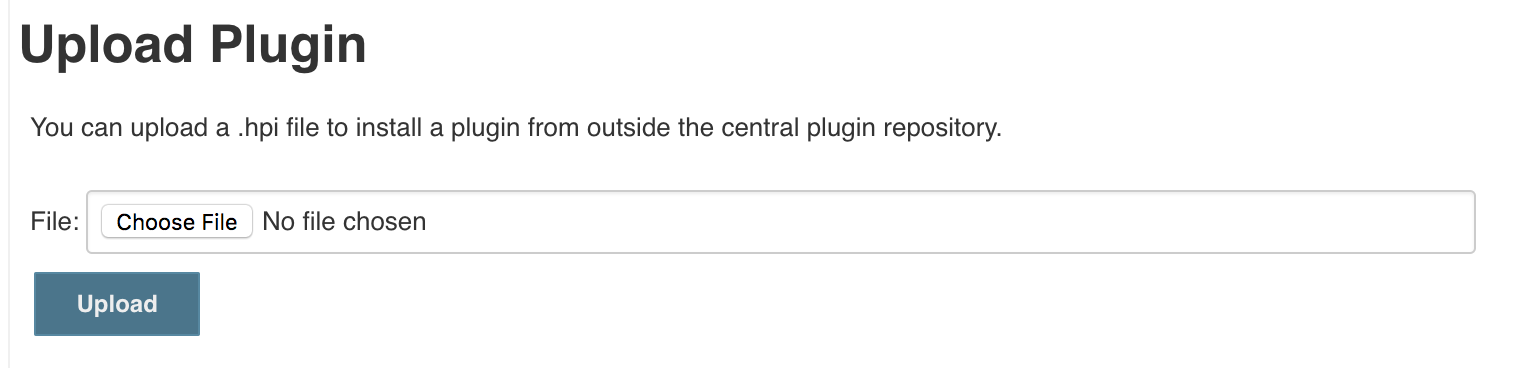
\includegraphics[width=0.9\textwidth]{grafiken/jenkins-plugin-03}
    \caption{Upload Plugin section}
    \label{fig:jenkins-plugin-03}
\end{figure}

There click on choose file and select the hpi file \textit{simile-jenkins-plugin.hpi} provided with the CD.
% \newpage
% \input{kapitel/methodologyQuestionMappingTable}
% 
% \input{kapitel/question_origins}
% \include{extern/fragebogenE}
% \include{extern/fragebogenD}
% 
% \input{kapitel/invitationLetters}
% 
% 
% \include{kapitel/coverageTable}

%Eidesstattliche Erklaerung
\chapter*{Eidesstattliche Erkl\"{a}rung}
\thispagestyle{empty}
Hiermit versichere ich, dass diese Abschlussarbeit von mir persönlich verfasst
ist und dass ich keinerlei fremde Hilfe in Anspruch genommen habe. Ebenso
versichere ich, dass diese Arbeit oder Teile daraus weder von mir selbst noch
von anderen als Leistungsnachweise andernorts eingereicht wurden. Wörtliche oder
sinn\-gemäße Übernahmen aus anderen Schriften und Veröffentlichungen in gedruckter
oder elektronischer Form sind gekennzeichnet. Sämtliche Sekundärliteratur und
sonstige Quellen sind nachgewiesen und in der Bibliographie aufgeführt. Das
Glei\-che gilt für graphische Darstellungen und Bilder sowie für alle
Internet-Quellen.

Ich bin ferner damit einverstanden, dass meine Arbeit zum Zwecke eines
Plagiatsabgleichs in elektronischer Form anonymisiert versendet und gespeichert
werden kann. Mir ist bekannt, dass von der Korrektur der Arbeit abgesehen werden
kann, wenn die Erklärung nicht erteilt wird.
\bigskip

\raggedright{Ort, den Datum} \bigskip \bigskip \bigskip

Martin Mustermann

\end{document}
